%!TEX root = ../dissertation.tex
\chapter{Constant \muqcd Validation}
\label{AppendixMuqcd}

\paragraph{}
One important assumption is the constant \muqcd for different regions on the 2D \mleadJ-\msublJ plane. 
This can be validated in data, excluding signal regions which were blinded during this check. 
The \ttbar~ contribution is estimated directly from MC and subtracted in the data distributions. 
The ratio of the number of n-$b$tagged events versus the number of less-$b$tagged events in each \mleadJ-\msublJ bin is calculated.
The pull of the ratios in SB/CR/SR is also calculated.
These two distributions shows the consistency of \muqcd in SB/CR/SR, as seen in Figure~\ref{fig:app-muqcd-1b} ($1b$ over $0b$), ~\ref{fig:app-muqcd-2b} ($2b$ over $1b$), ~\ref{fig:app-muqcd-2bs} ($2bs$ over $1b$), ~\ref{fig:app-muqcd-3b} ($3b$ over $2b$), ~\ref{fig:app-muqcd-4b} ($4b$ over $2b$). For $4/3/2bs$, the \muqcd value can be compared with \ref{tab:bkgfit}. 
This validates the choice of SB region and the constant \muqcd assumption in the analysis.

\begin{figure*}[htbp!]
\begin{center}
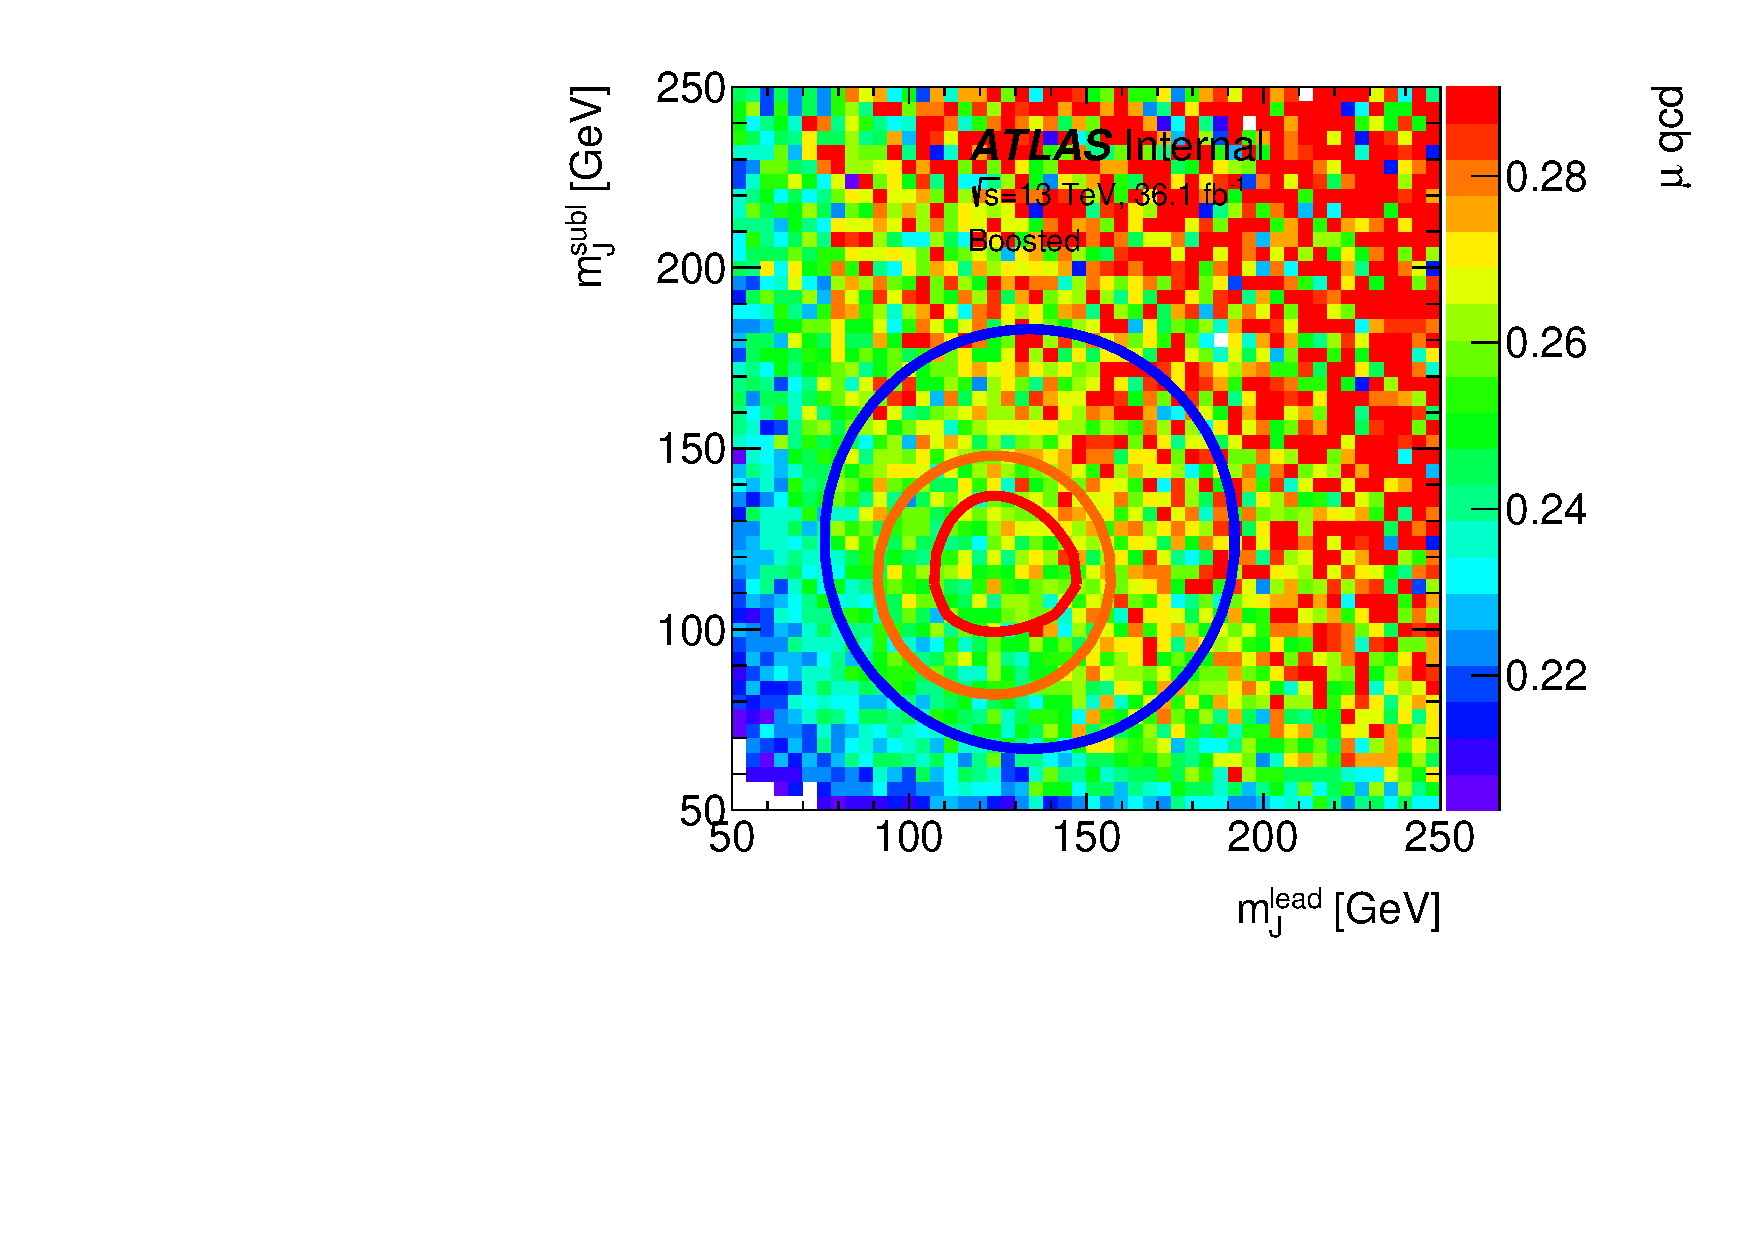
\includegraphics[width=0.31\textwidth,angle=-90]{figures/boosted/AppendixMuqcdstudy/OneTag_Incl_mH0H1.pdf}
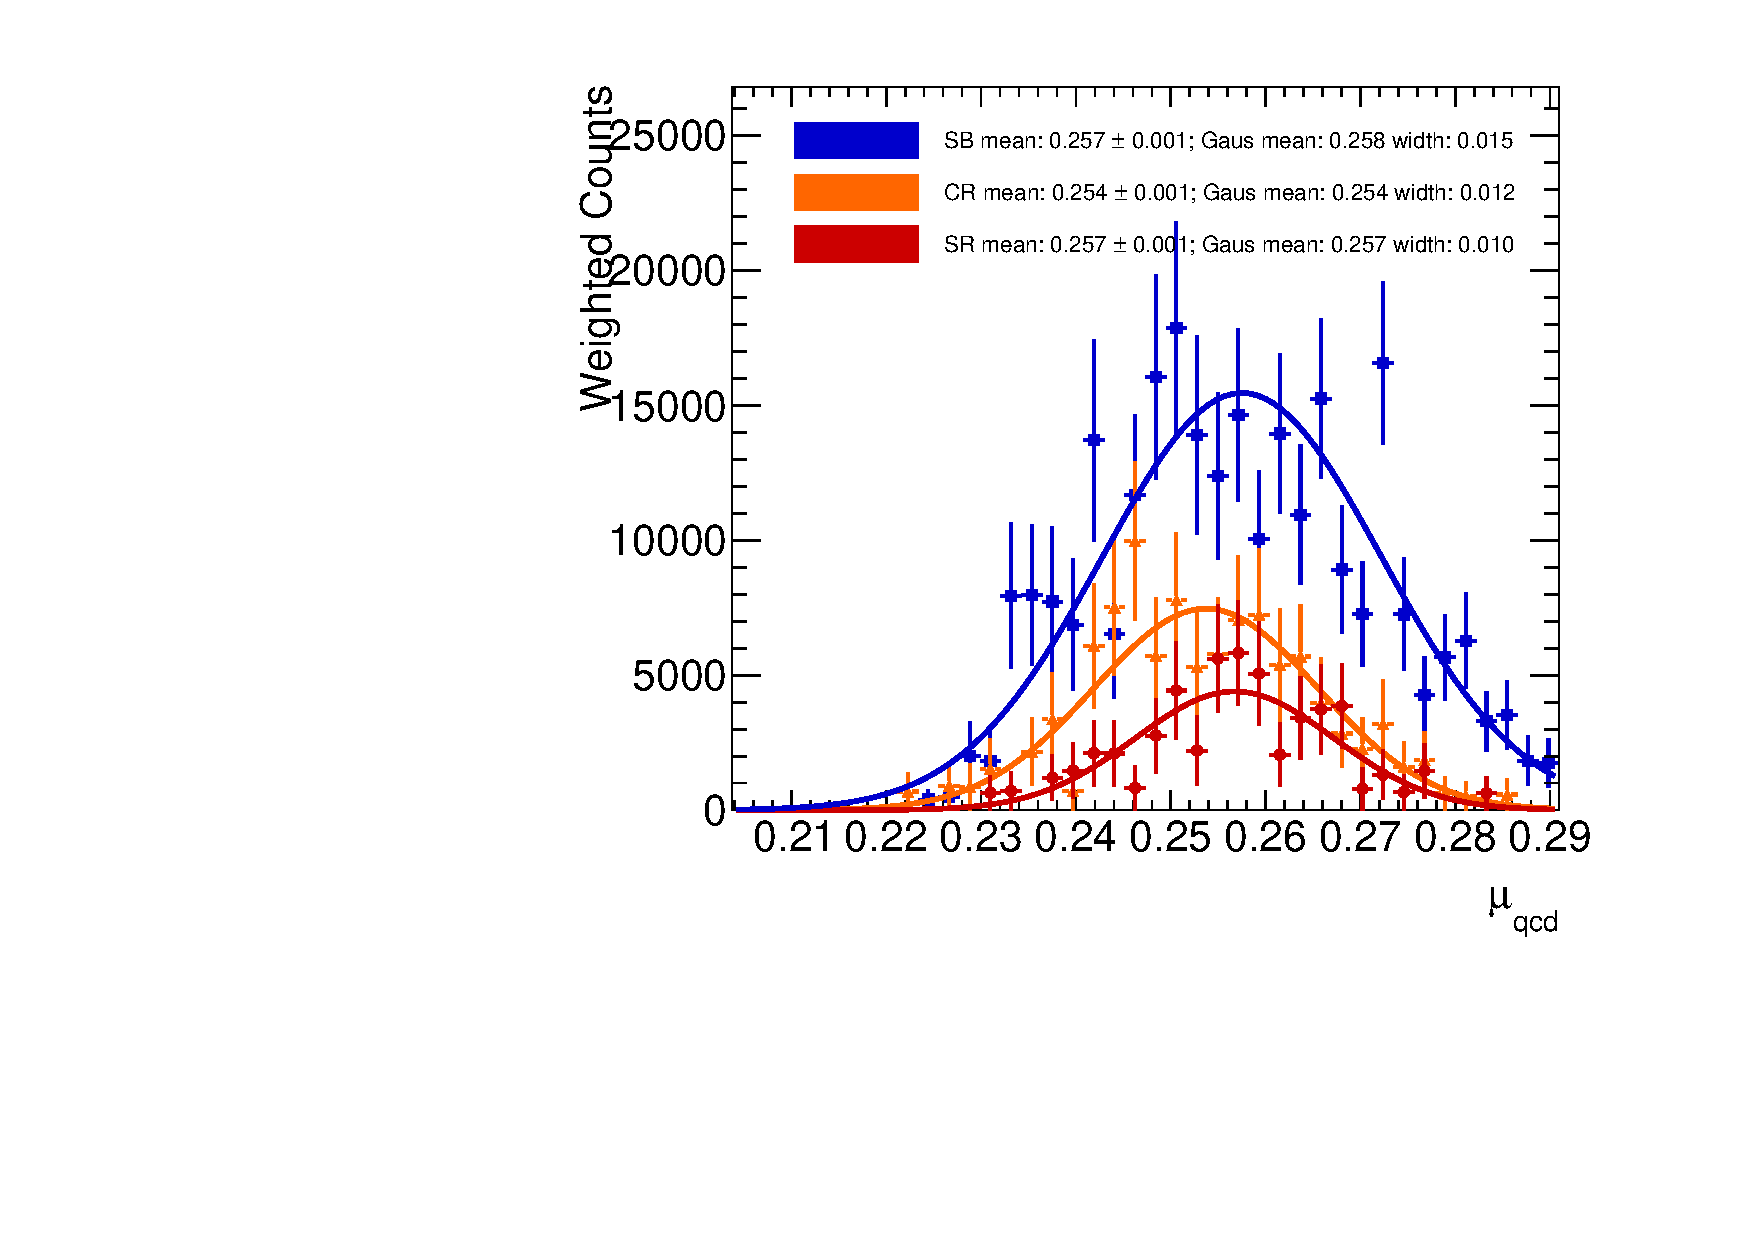
\includegraphics[width=0.31\textwidth,angle=-90]{figures/boosted/AppendixMuqcdstudy/OneTag_Incl_mH0H1_pull.pdf}
\caption{$1b$ over 0$b$ \muqcd~ values: \muqcd variations on 2D \mleadJ-msublJ plane(left); and \muqcd pull distribution in SB/CR/SR(right), with the $N_{event}$ weighted mean value and the Gaussian fit mean value shown on the plot.}
\label{fig:app-muqcd-1b}
\end{center}
\end{figure*}

\begin{figure*}[htbp!]
\begin{center}
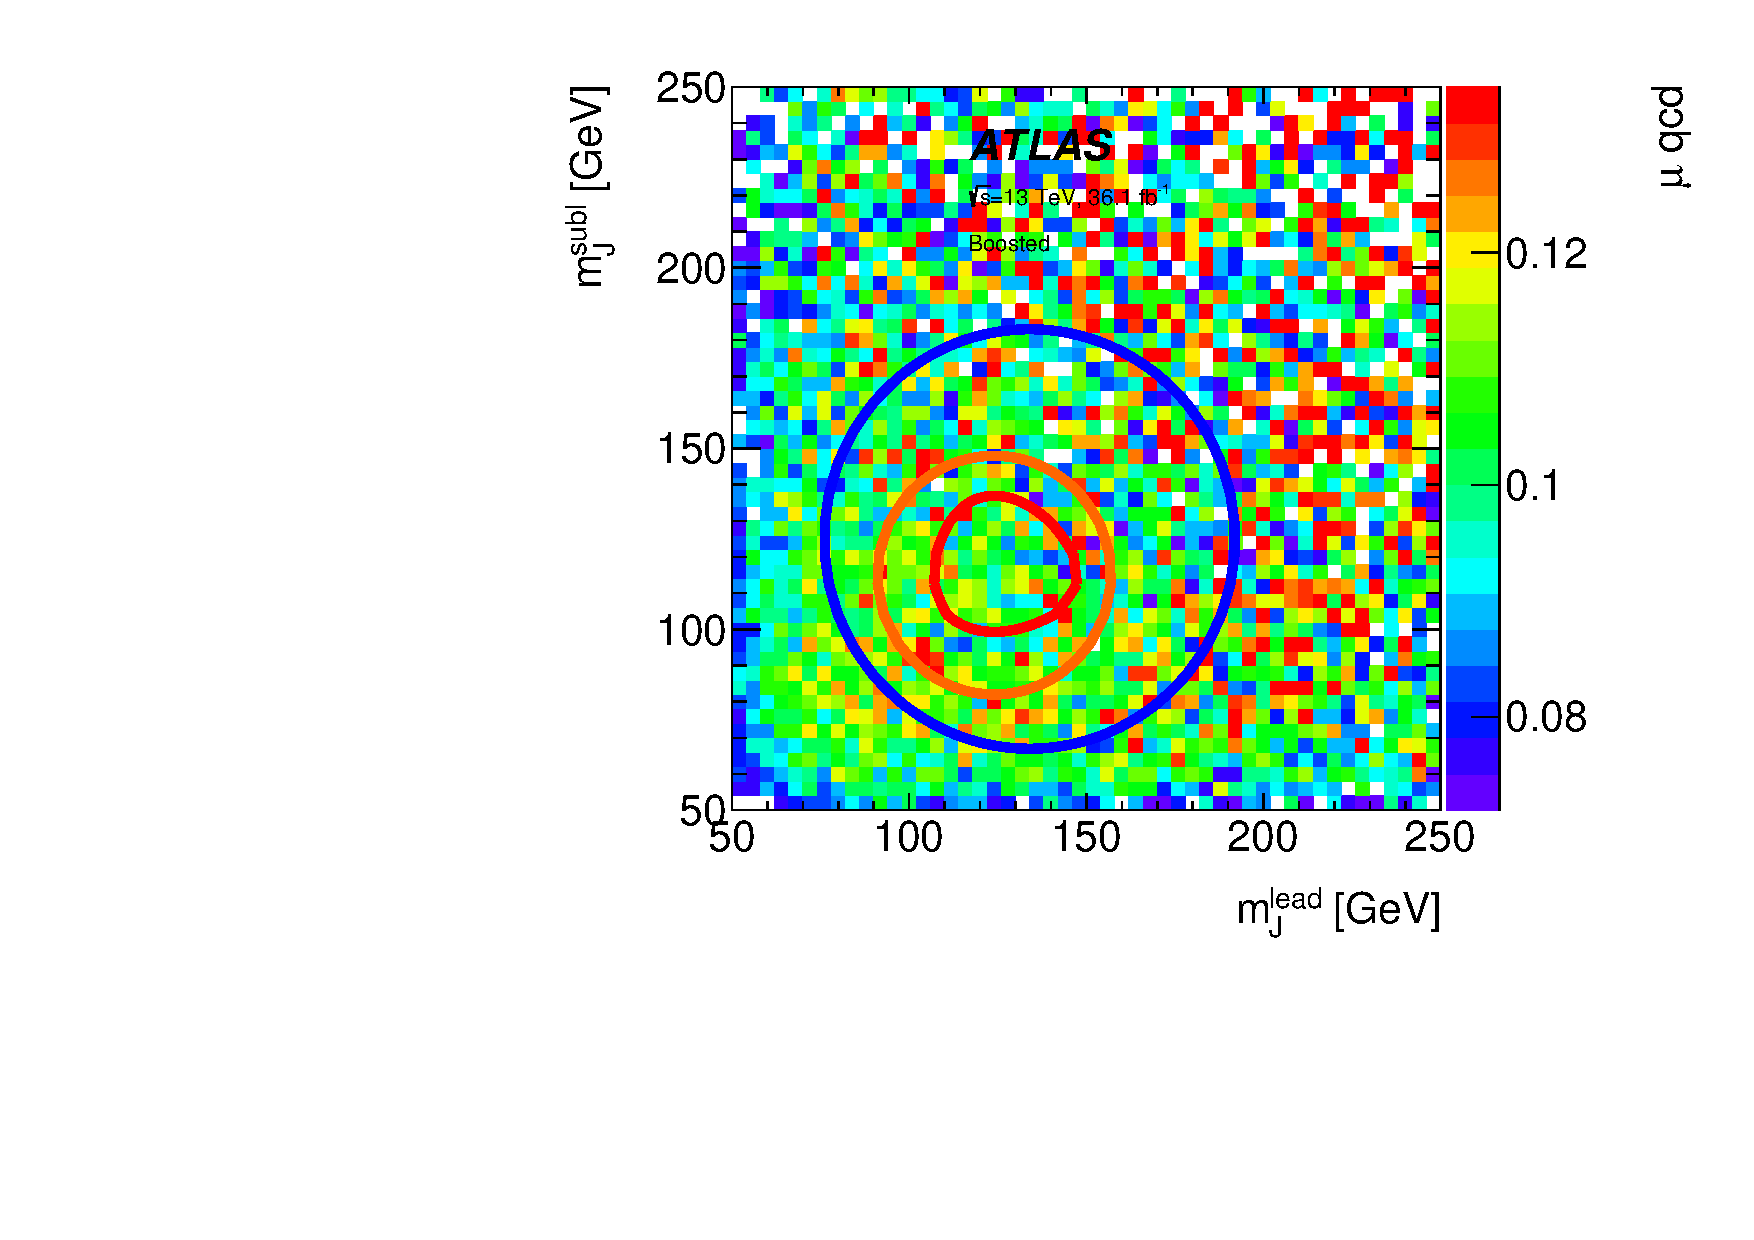
\includegraphics[width=0.31\textwidth,angle=-90]{figures/boosted/AppendixMuqcdstudy/TwoTag_Incl_mH0H1.pdf}
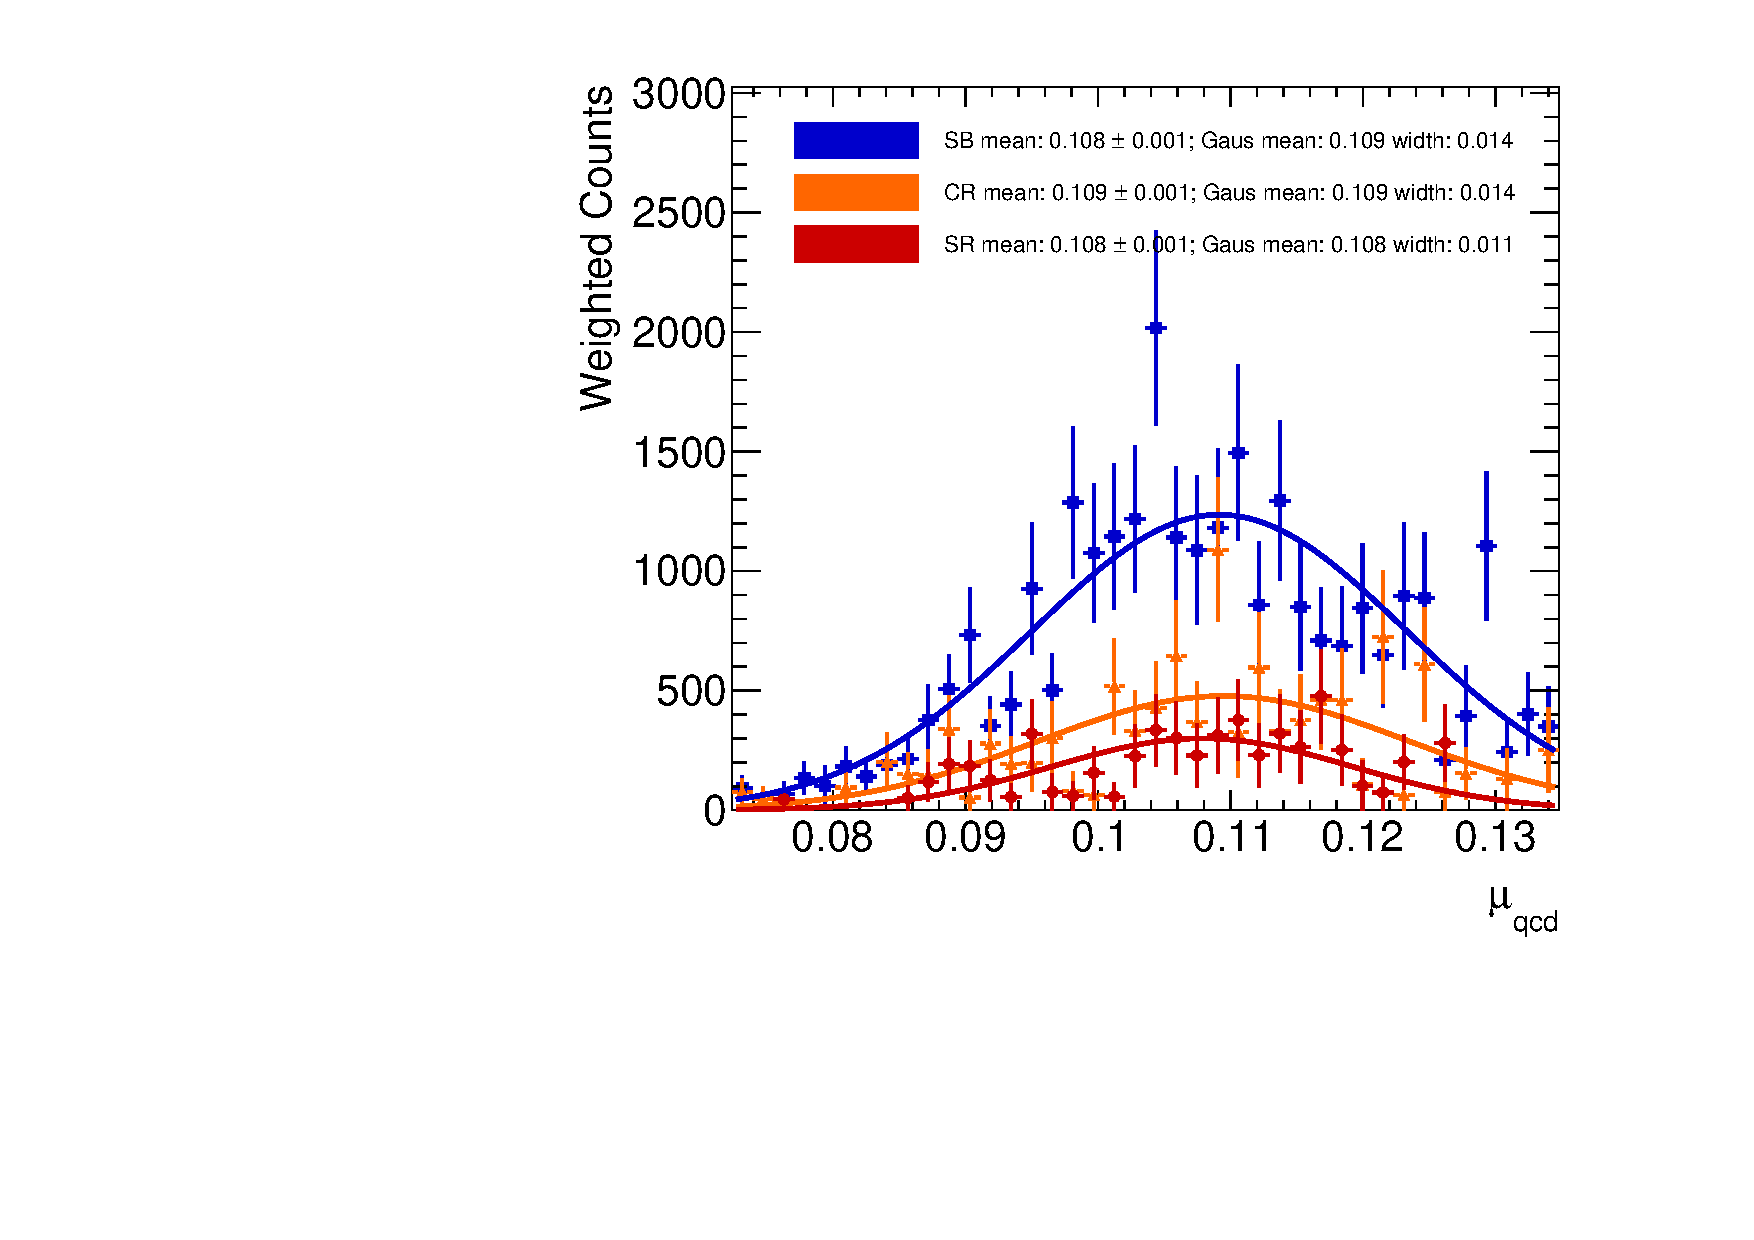
\includegraphics[width=0.31\textwidth,angle=-90]{figures/boosted/AppendixMuqcdstudy/TwoTag_Incl_mH0H1_pull.pdf}
\caption{$2b$ over $1b$ \muqcd~ values: \muqcd variations on 2D \mleadJ-msublJ plane(left); and \muqcd pull distribution in SB/CR/SR(right), with the $N_{event}$ weighted mean value and the Gaussian fit mean value shown on the plot.}
\label{fig:app-muqcd-2b}
\end{center}
\end{figure*}

\begin{figure*}[htbp!]
\begin{center}
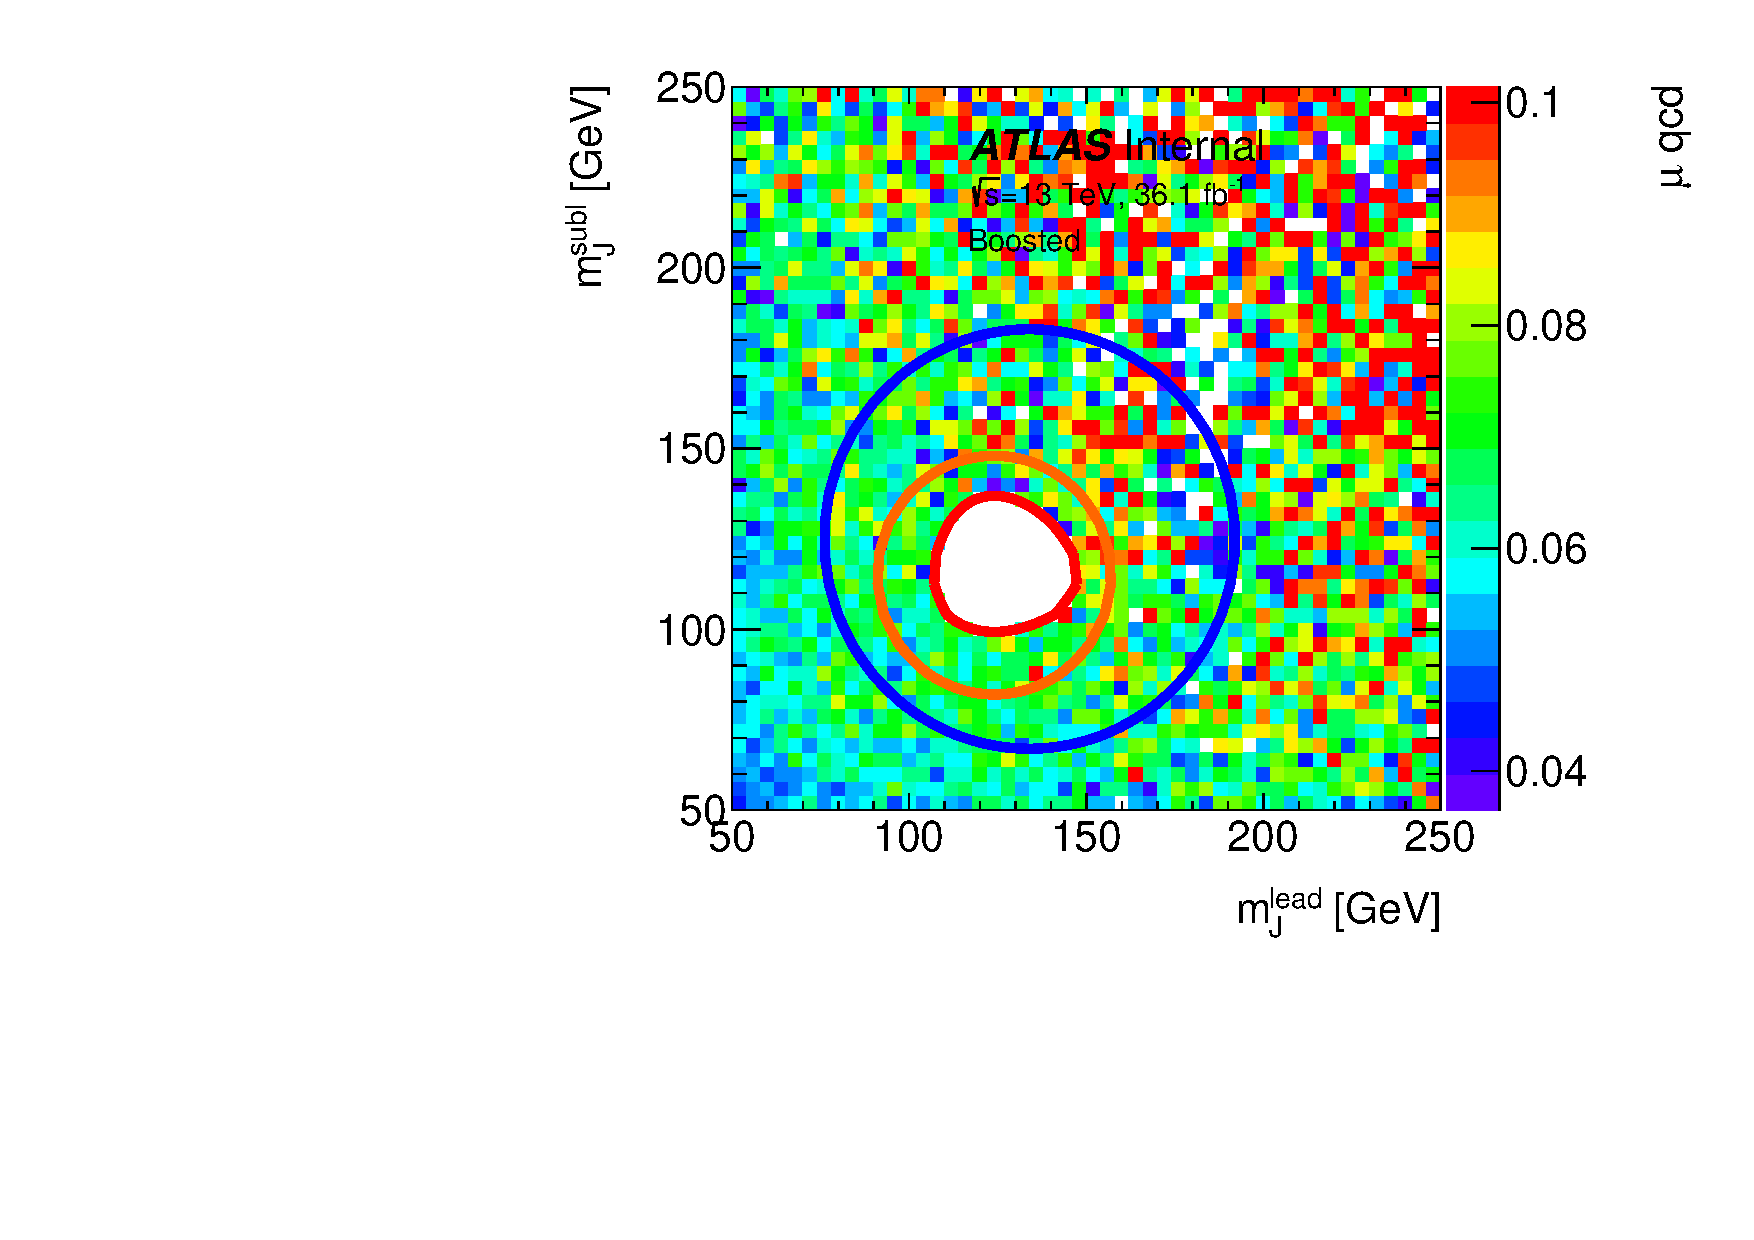
\includegraphics[width=0.31\textwidth,angle=-90]{figures/boosted/AppendixMuqcdstudy/TwoTag_split_Incl_mH0H1.pdf}
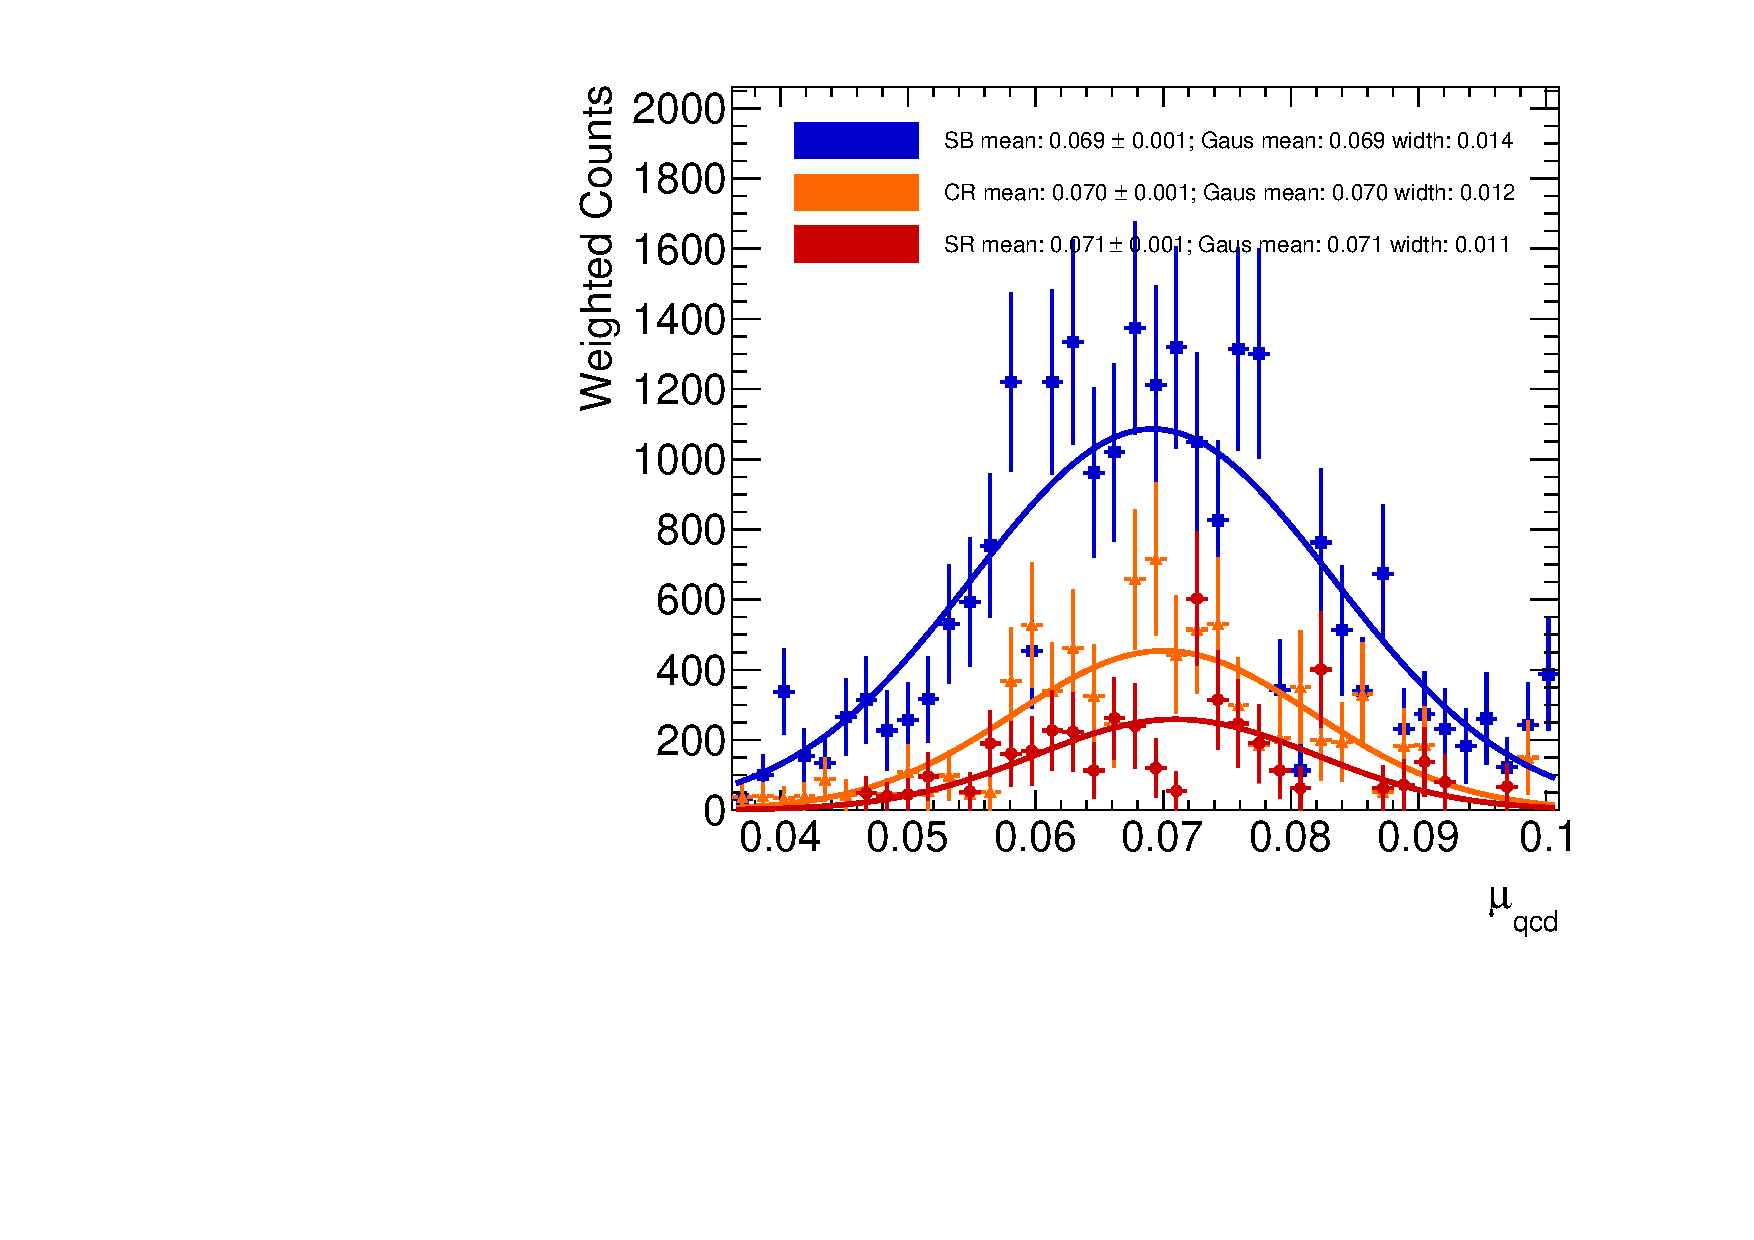
\includegraphics[width=0.31\textwidth,angle=-90]{figures/boosted/AppendixMuqcdstudy/TwoTag_split_Incl_mH0H1_pull.pdf}
\caption{$2bs$ over $1b$ \muqcd~ values: \muqcd variations on 2D \mleadJ-msublJ plane(left); and \muqcd pull distribution in SB/CR/SR(right), with the $N_{event}$ weighted mean value and the Gaussian fit mean value shown on the plot.}
\label{fig:app-muqcd-2bs}
\end{center}
\end{figure*}

\begin{figure*}[htbp!]
\begin{center}
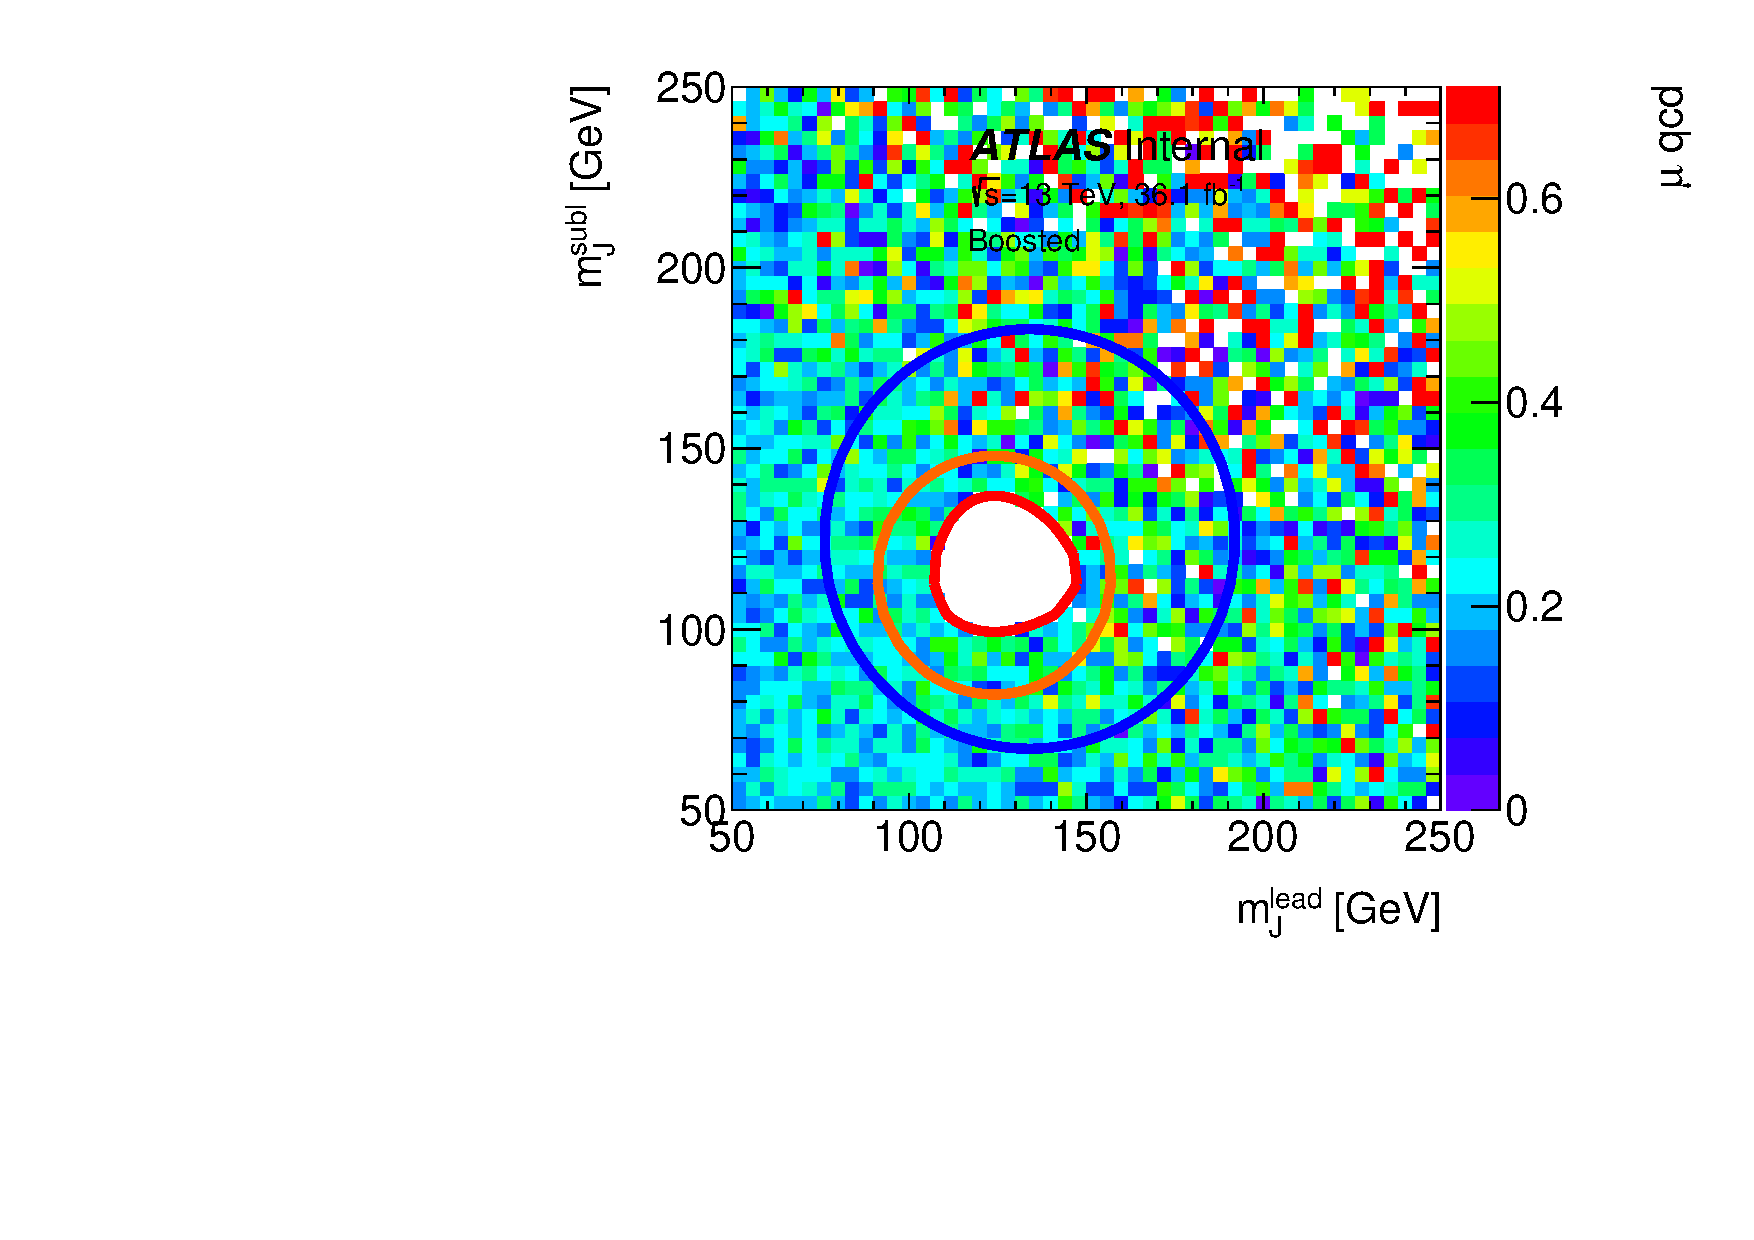
\includegraphics[width=0.31\textwidth,angle=-90]{figures/boosted/AppendixMuqcdstudy/ThreeTag_Incl_mH0H1.pdf}
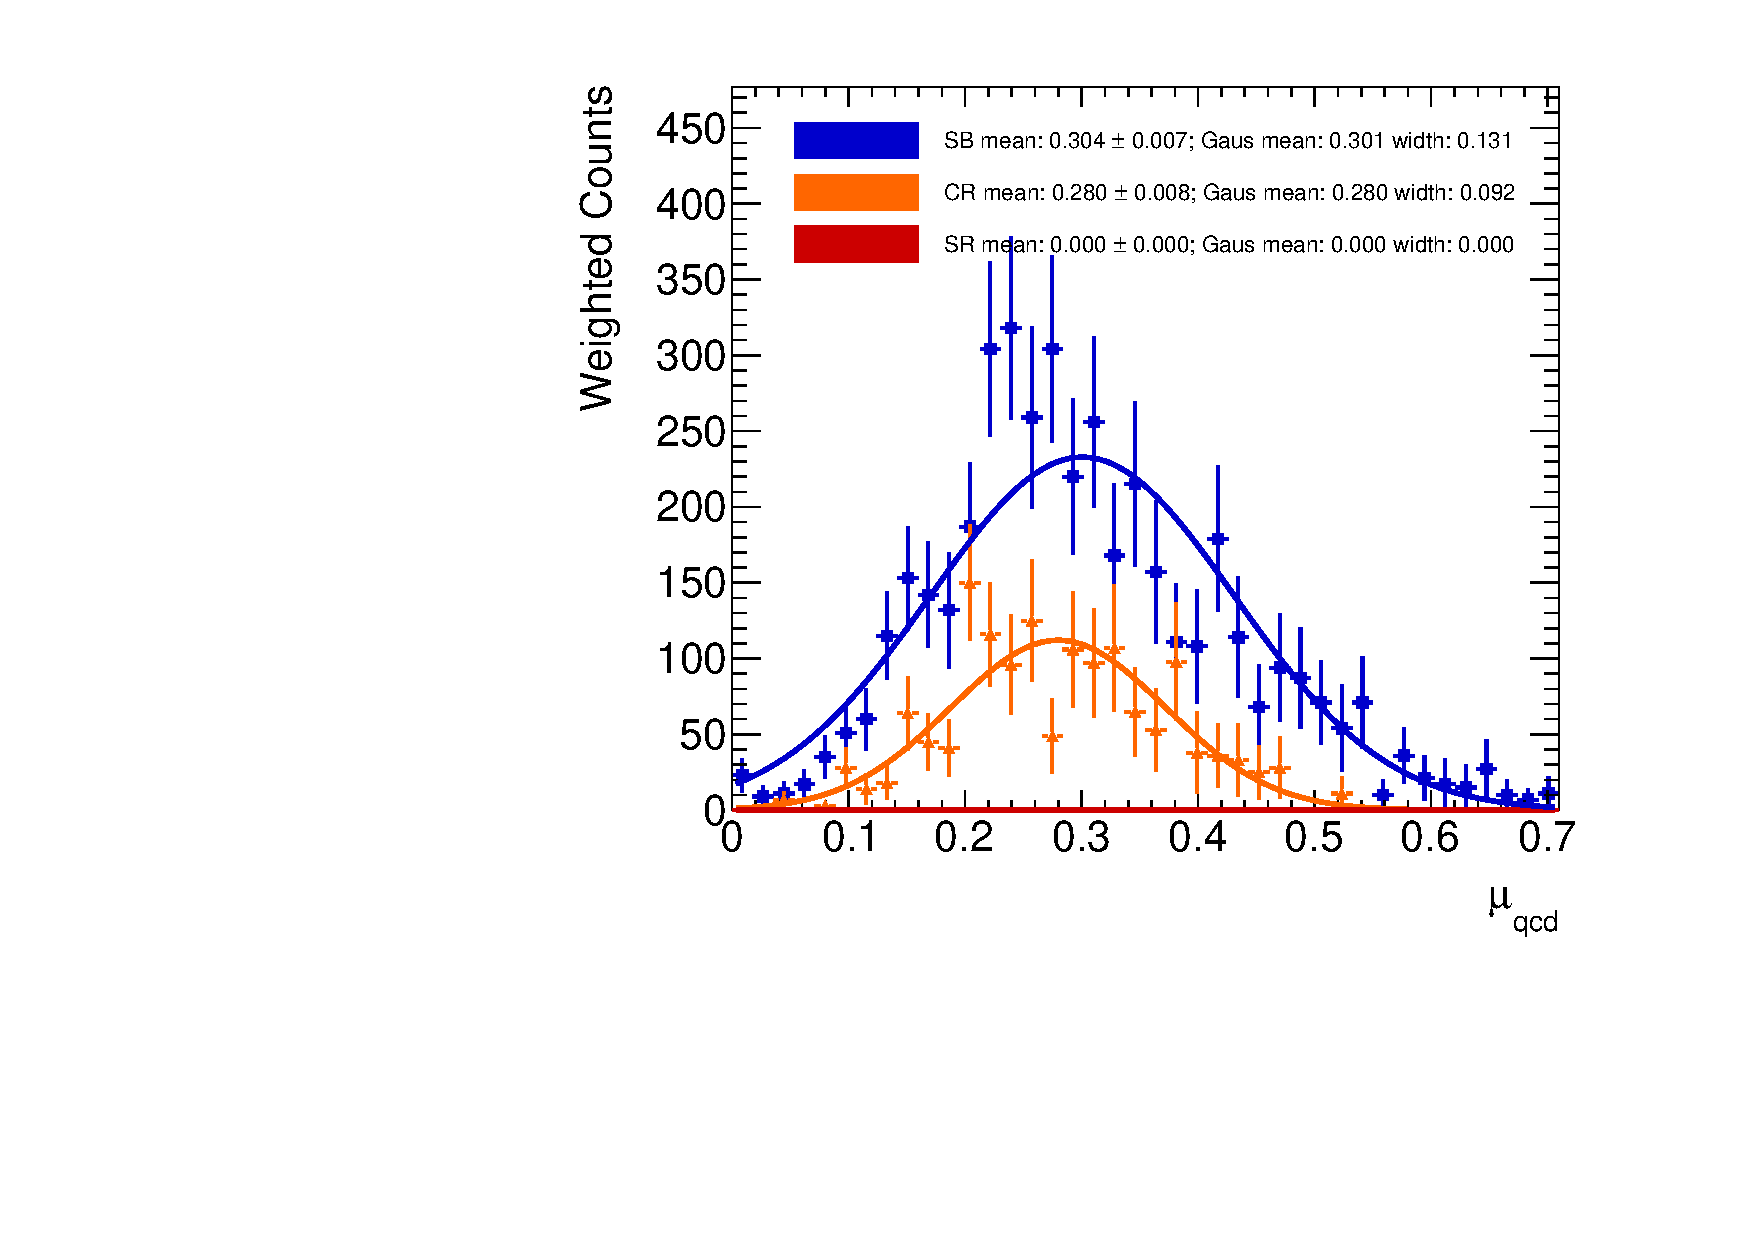
\includegraphics[width=0.31\textwidth,angle=-90]{figures/boosted/AppendixMuqcdstudy/ThreeTag_Incl_mH0H1_pull.pdf}
\caption{$3b$ over $2b$ \muqcd~ values: \muqcd variations on 2D \mleadJ-msublJ plane(left); and \muqcd pull distribution in SB/CR/SR(right), with the $N_{event}$ weighted mean value and the Gaussian fit mean value shown on the plot.}
\label{fig:app-muqcd-3b}
\end{center}
\end{figure*}

\begin{figure*}[htbp!]
\begin{center}
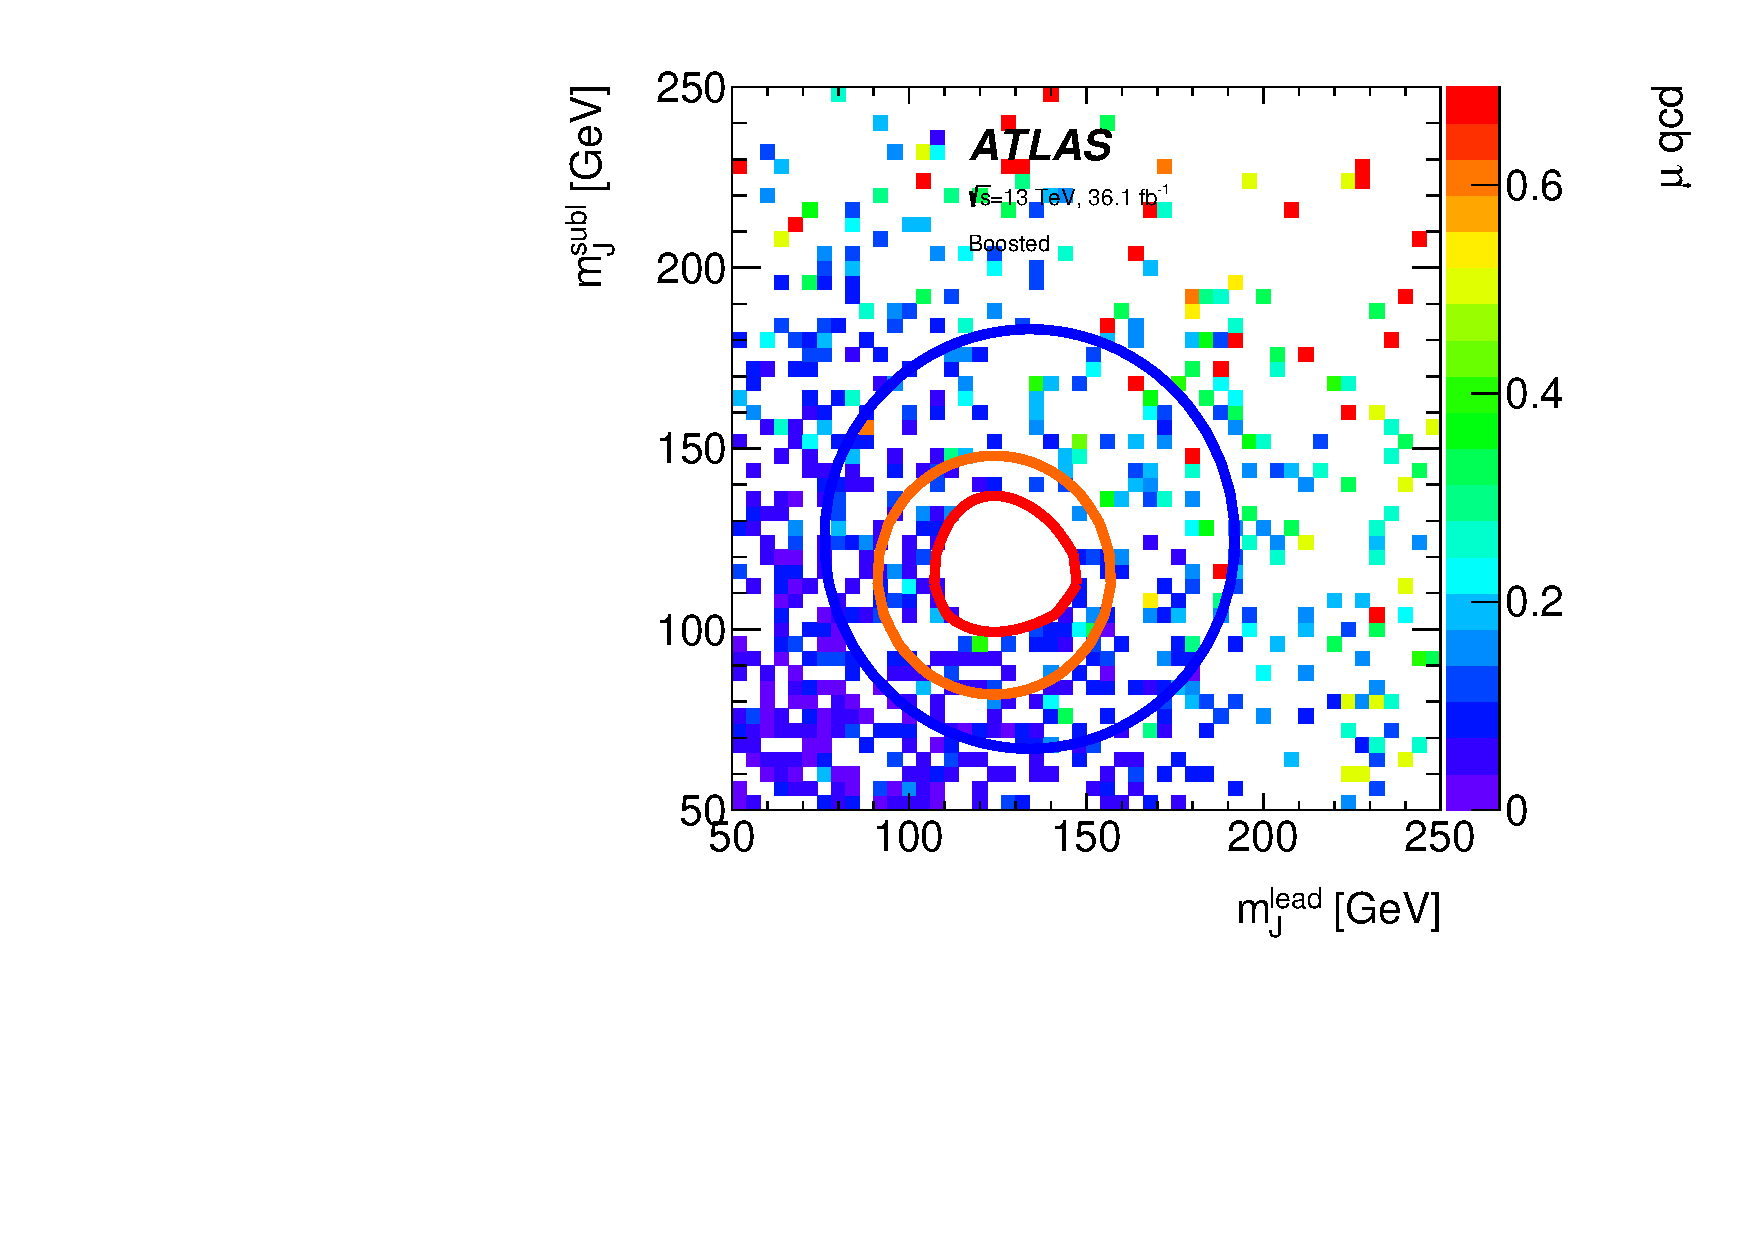
\includegraphics[width=0.31\textwidth,angle=-90]{figures/boosted/AppendixMuqcdstudy/FourTag_Incl_mH0H1.pdf}
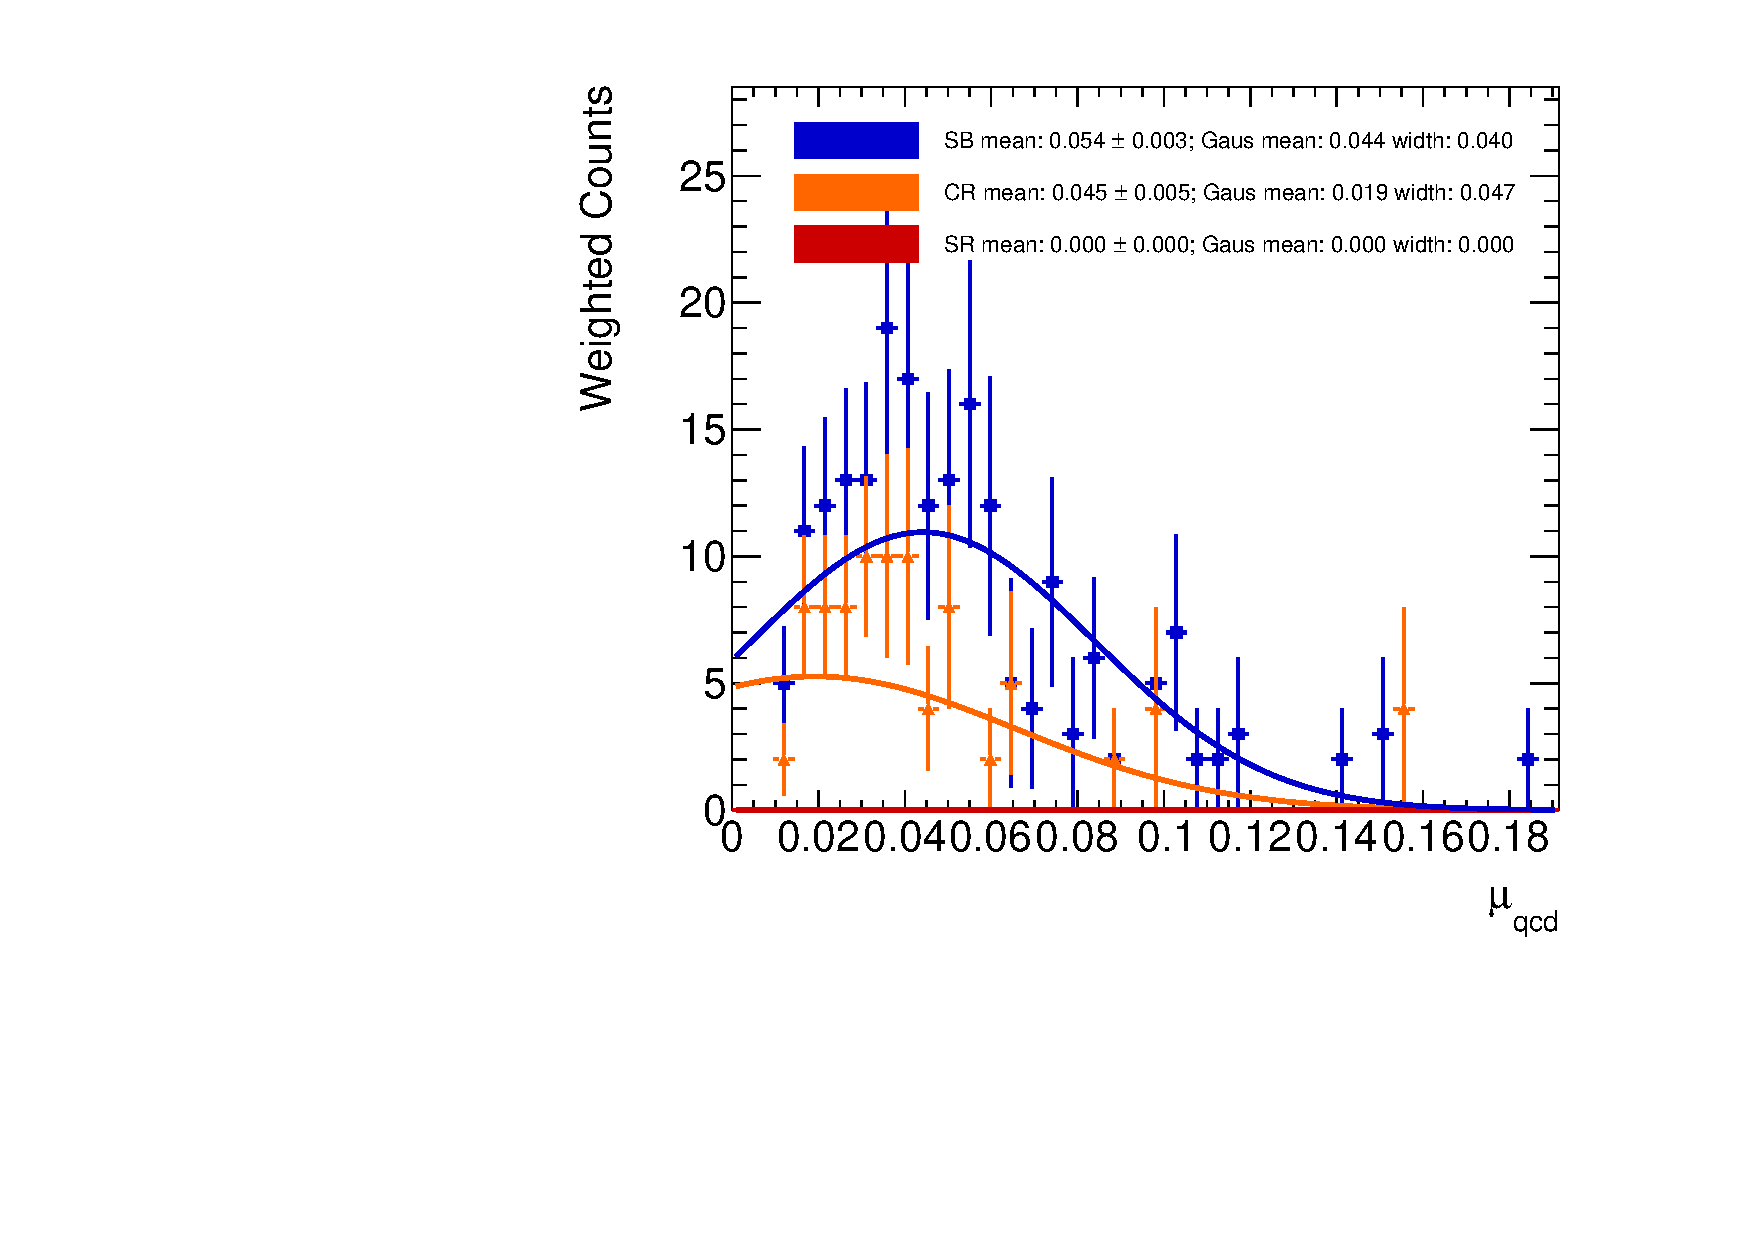
\includegraphics[width=0.31\textwidth,angle=-90]{figures/boosted/AppendixMuqcdstudy/FourTag_Incl_mH0H1_pull.pdf}
\caption{$4b$ over $2b$ \muqcd~ values: \muqcd variations on 2D \mleadJ-msublJ plane(left); and \muqcd pull distribution in SB/CR/SR(right), with the $N_{event}$ weighted mean value and the Gaussian fit mean value shown on the plot.}
\label{fig:app-muqcd-4b}
\end{center}
\end{figure*}

\paragraph{}
Also, the Dijet MC can be used for validation. 
The same distributions evaluated in dijet MC are shown in Figure~\ref{fig:app-muqcd-1b-qcd} ($1b$ over $0b$), ~\ref{fig:app-muqcd-2b-qcd} ($2b$ over $1b$), ~\ref{fig:app-muqcd-2bs-qcd} ($2bs$ over $1b$), ~\ref{fig:app-muqcd-3b-qcd} ($3b$ over $2b$), ~\ref{fig:app-muqcd-4b-qcd} ($4b$ over $2b$).  
Poor Statistics of the dijet MC affect the pull distributions, yet the consistency of \muqcd in different regions can still be validated.
This also shows that the dijet MC could not be used directly for background estimation.


\begin{figure*}[htbp!]
\begin{center}
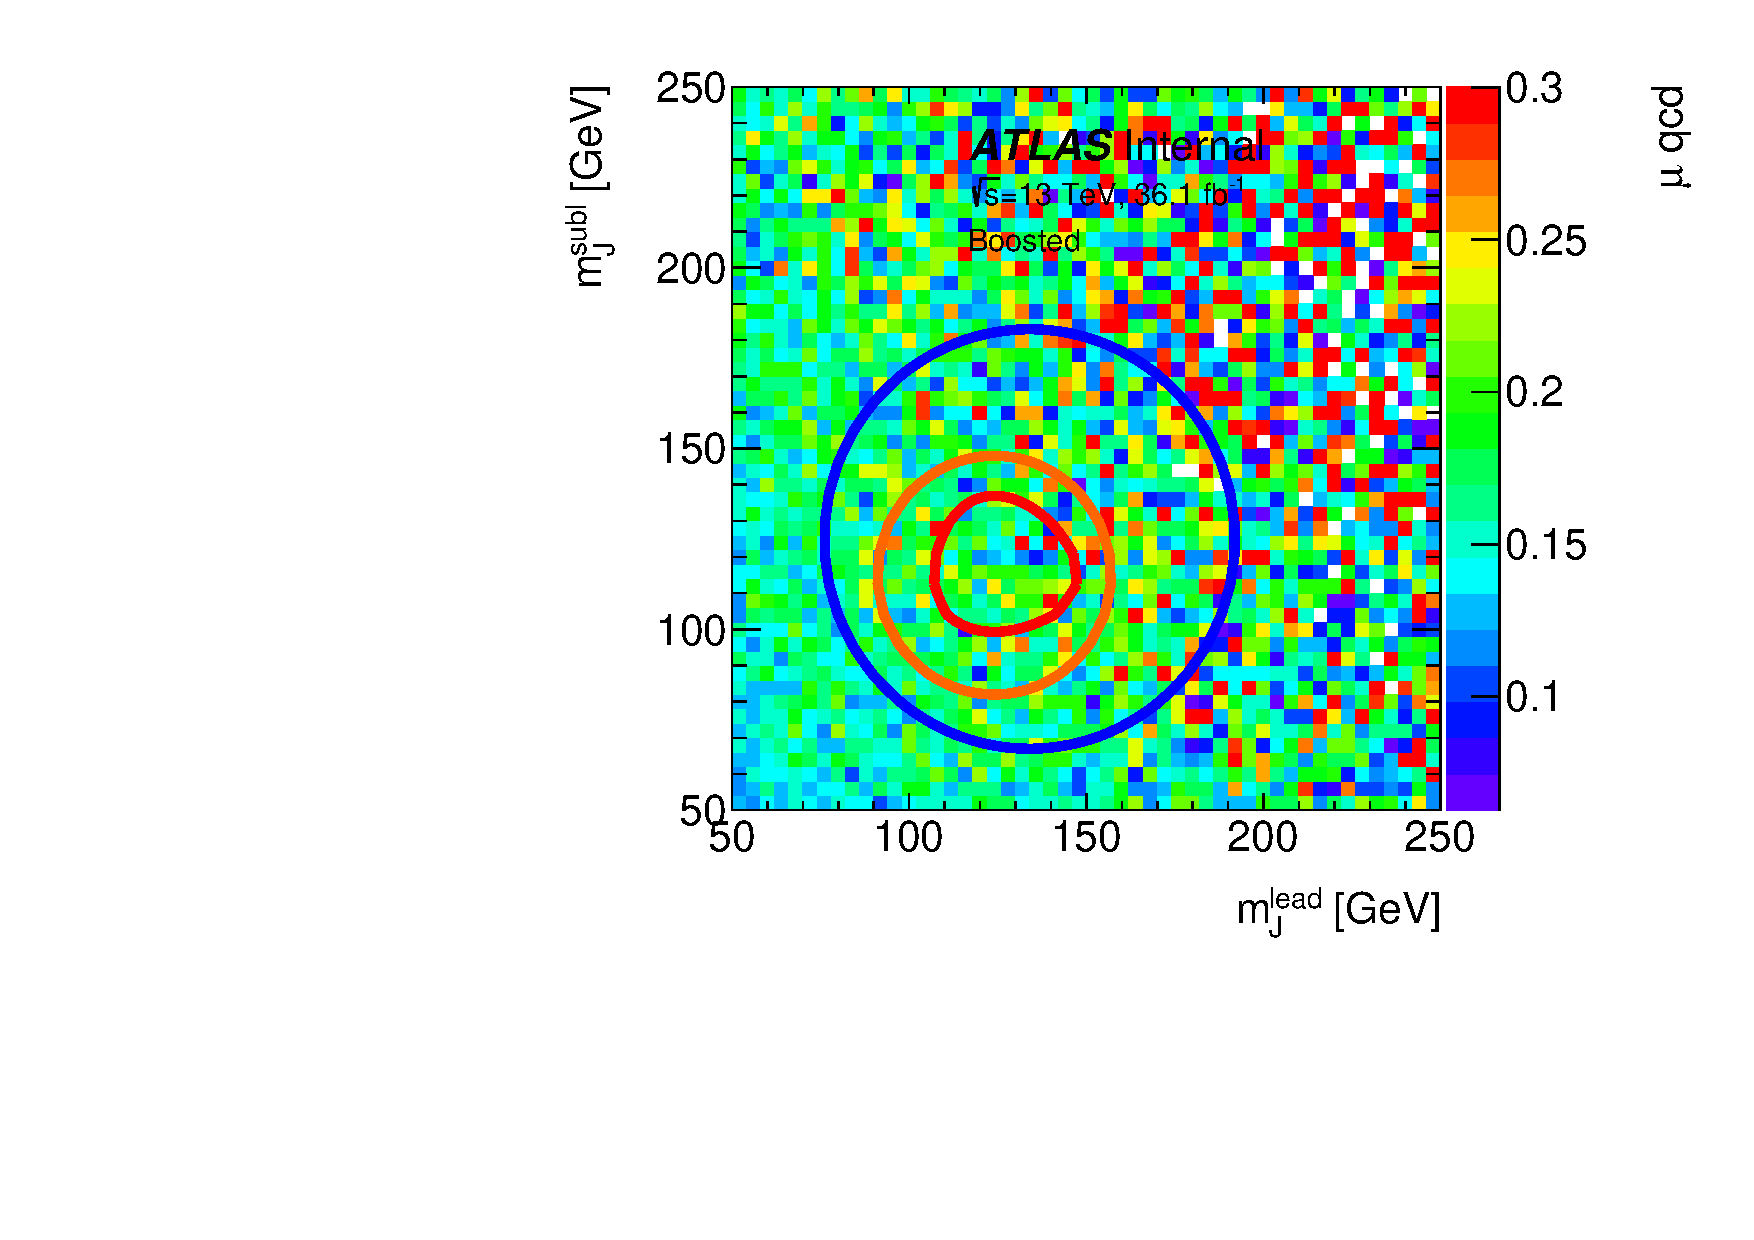
\includegraphics[width=0.31\textwidth,angle=-90]{figures/boosted/AppendixMuqcdstudy/QCD_OneTag_Incl_mH0H1.pdf}
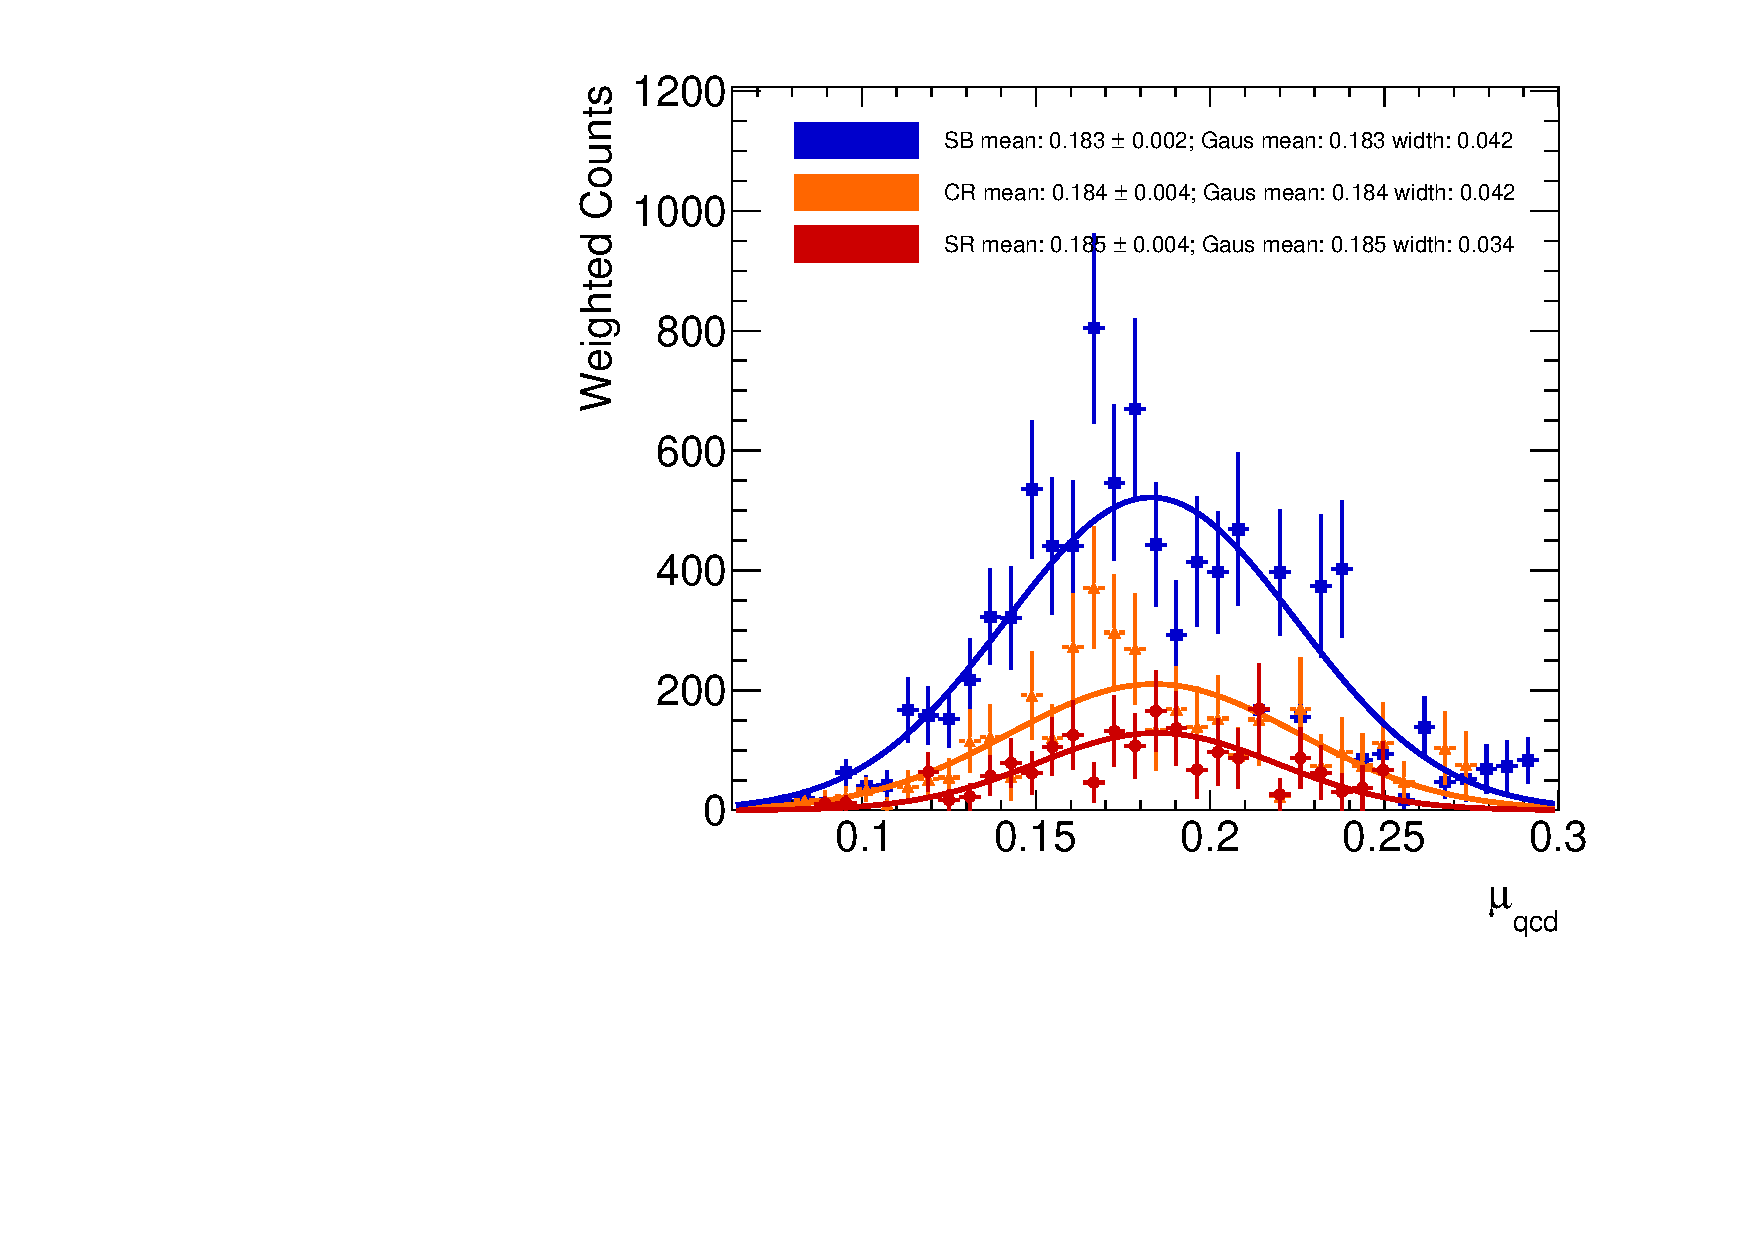
\includegraphics[width=0.31\textwidth,angle=-90]{figures/boosted/AppendixMuqcdstudy/QCD_OneTag_Incl_mH0H1_pull.pdf}
\caption{$1b$ over 0$b$ \muqcd~ values in dijet MC: \muqcd variations on 2D \mleadJ-msublJ plane(left); and \muqcd pull distribution in SB/CR/SR(right), with the $N_{event}$ weighted mean value and the Guassian fit mean value shown on the plot.}
\label{fig:app-muqcd-1b-qcd}
\end{center}
\end{figure*}

\begin{figure*}[htbp!]
\begin{center}
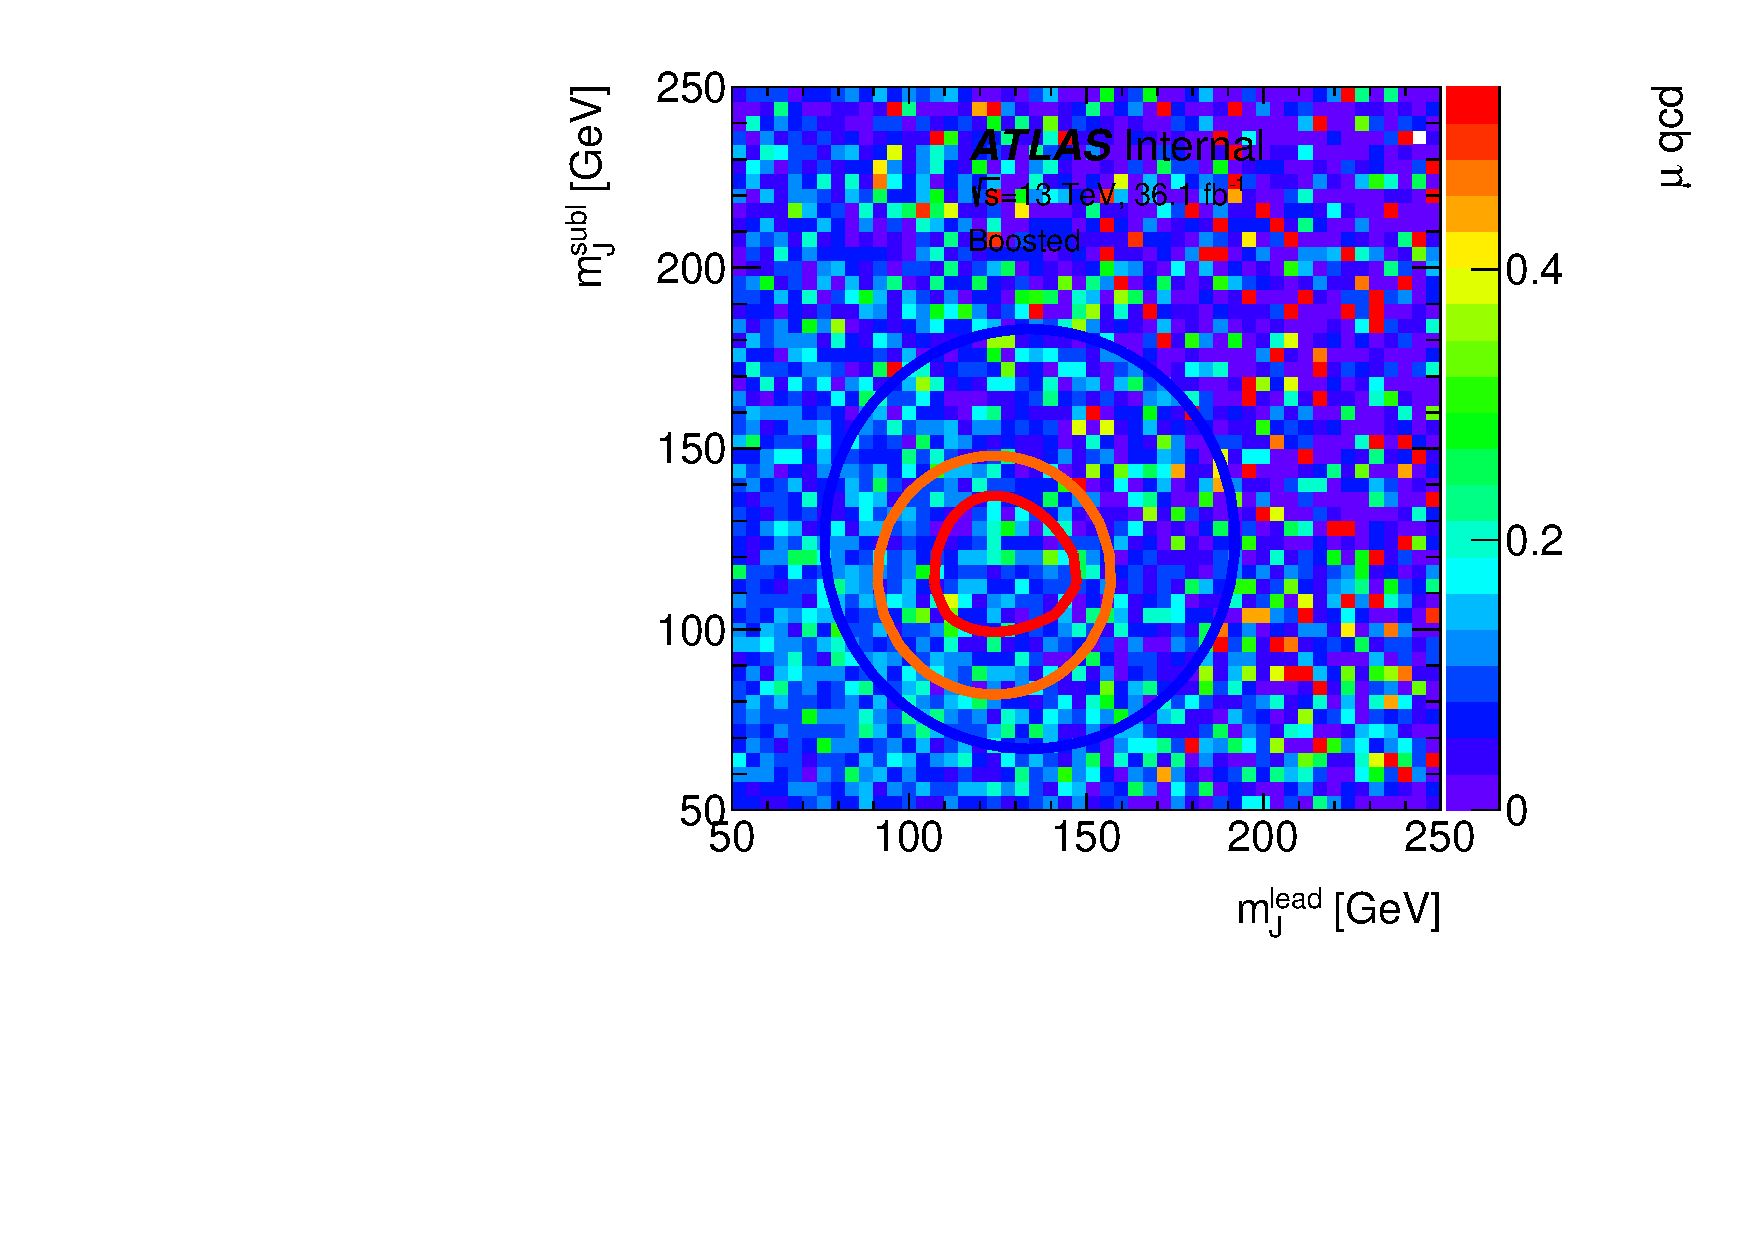
\includegraphics[width=0.31\textwidth,angle=-90]{figures/boosted/AppendixMuqcdstudy/QCD_TwoTag_Incl_mH0H1.pdf}
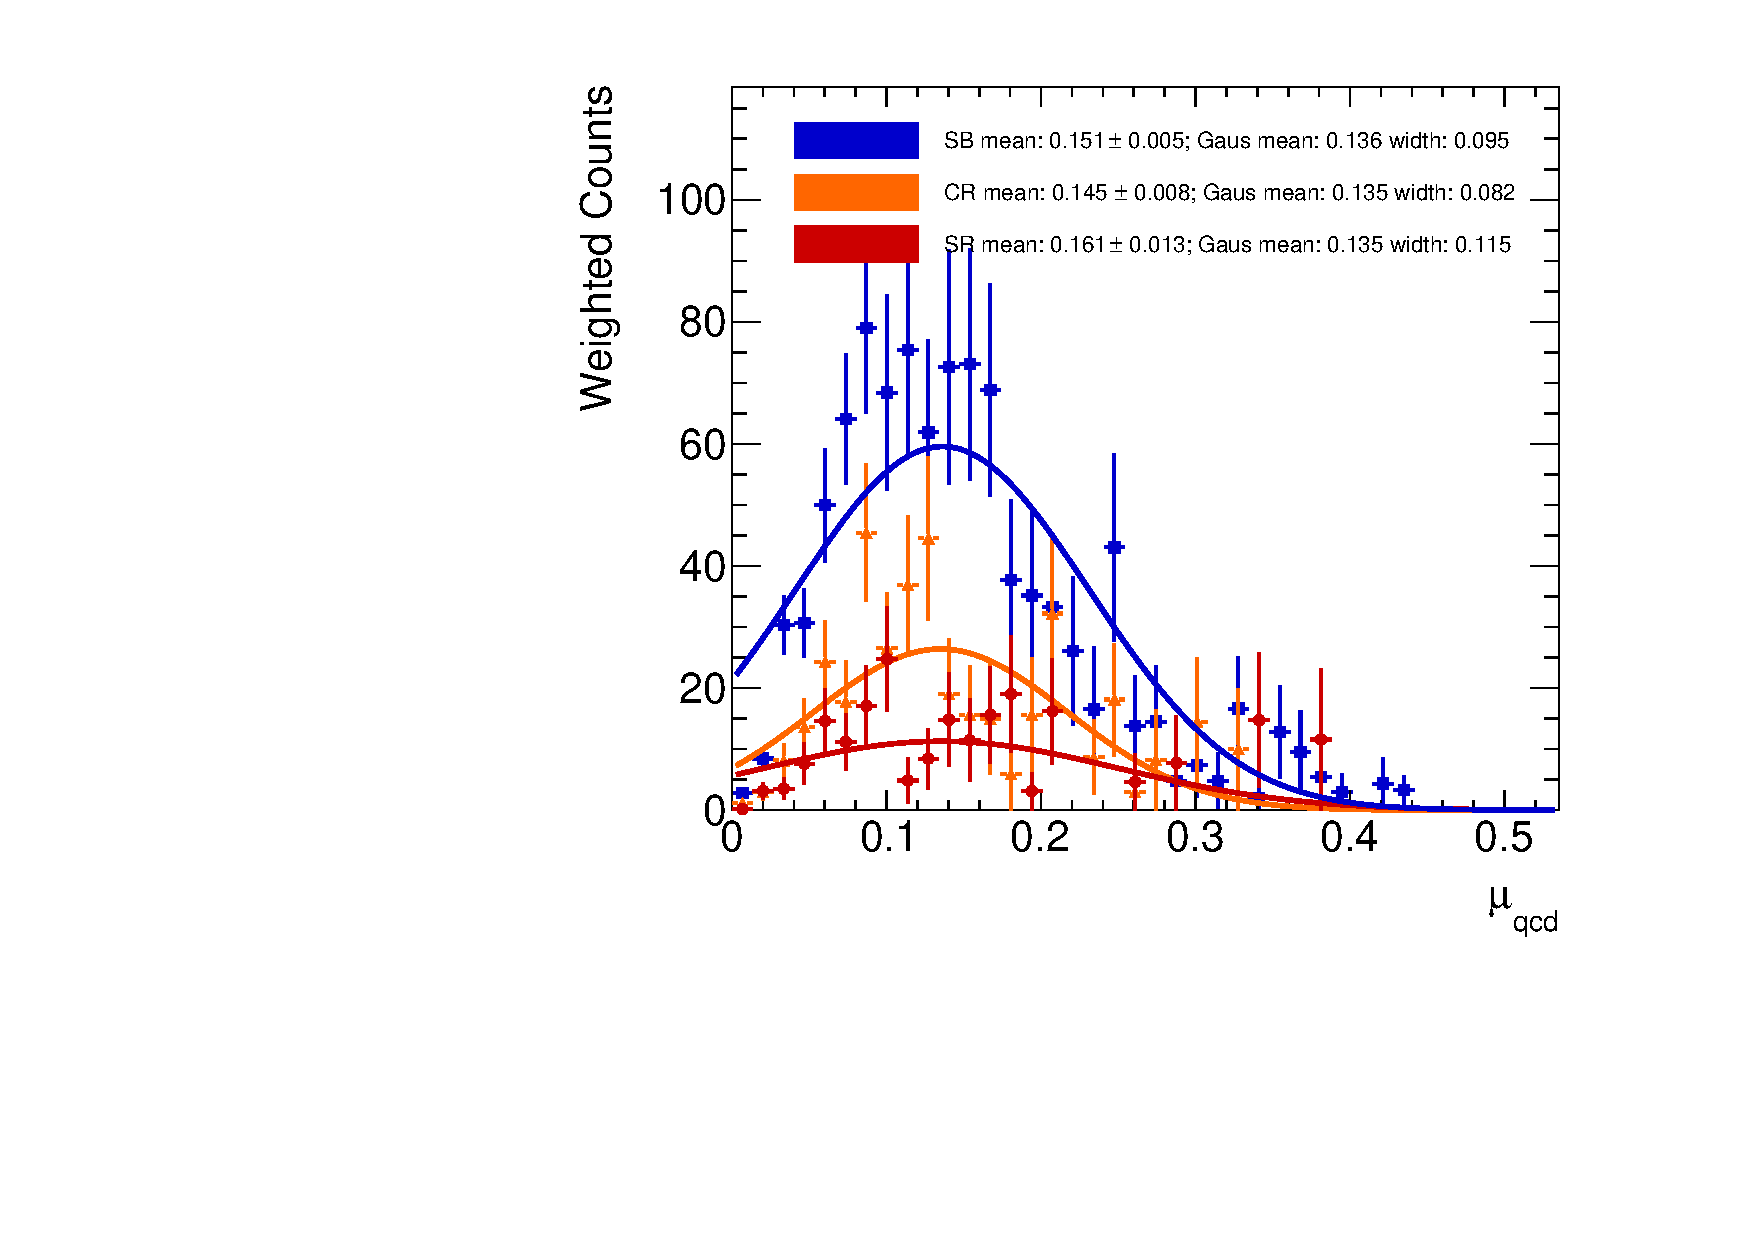
\includegraphics[width=0.31\textwidth,angle=-90]{figures/boosted/AppendixMuqcdstudy/QCD_TwoTag_Incl_mH0H1_pull.pdf}
\caption{$2b$ over $1b$ \muqcd~ values in dijet MC: \muqcd variations on 2D \mleadJ-msublJ plane(left); and \muqcd pull distribution in SB/CR/SR(right), with the $N_{event}$ weighted mean value and the Guassian fit mean value shown on the plot.}
\label{fig:app-muqcd-2b-qcd}
\end{center}
\end{figure*}

\begin{figure*}[htbp!]
\begin{center}
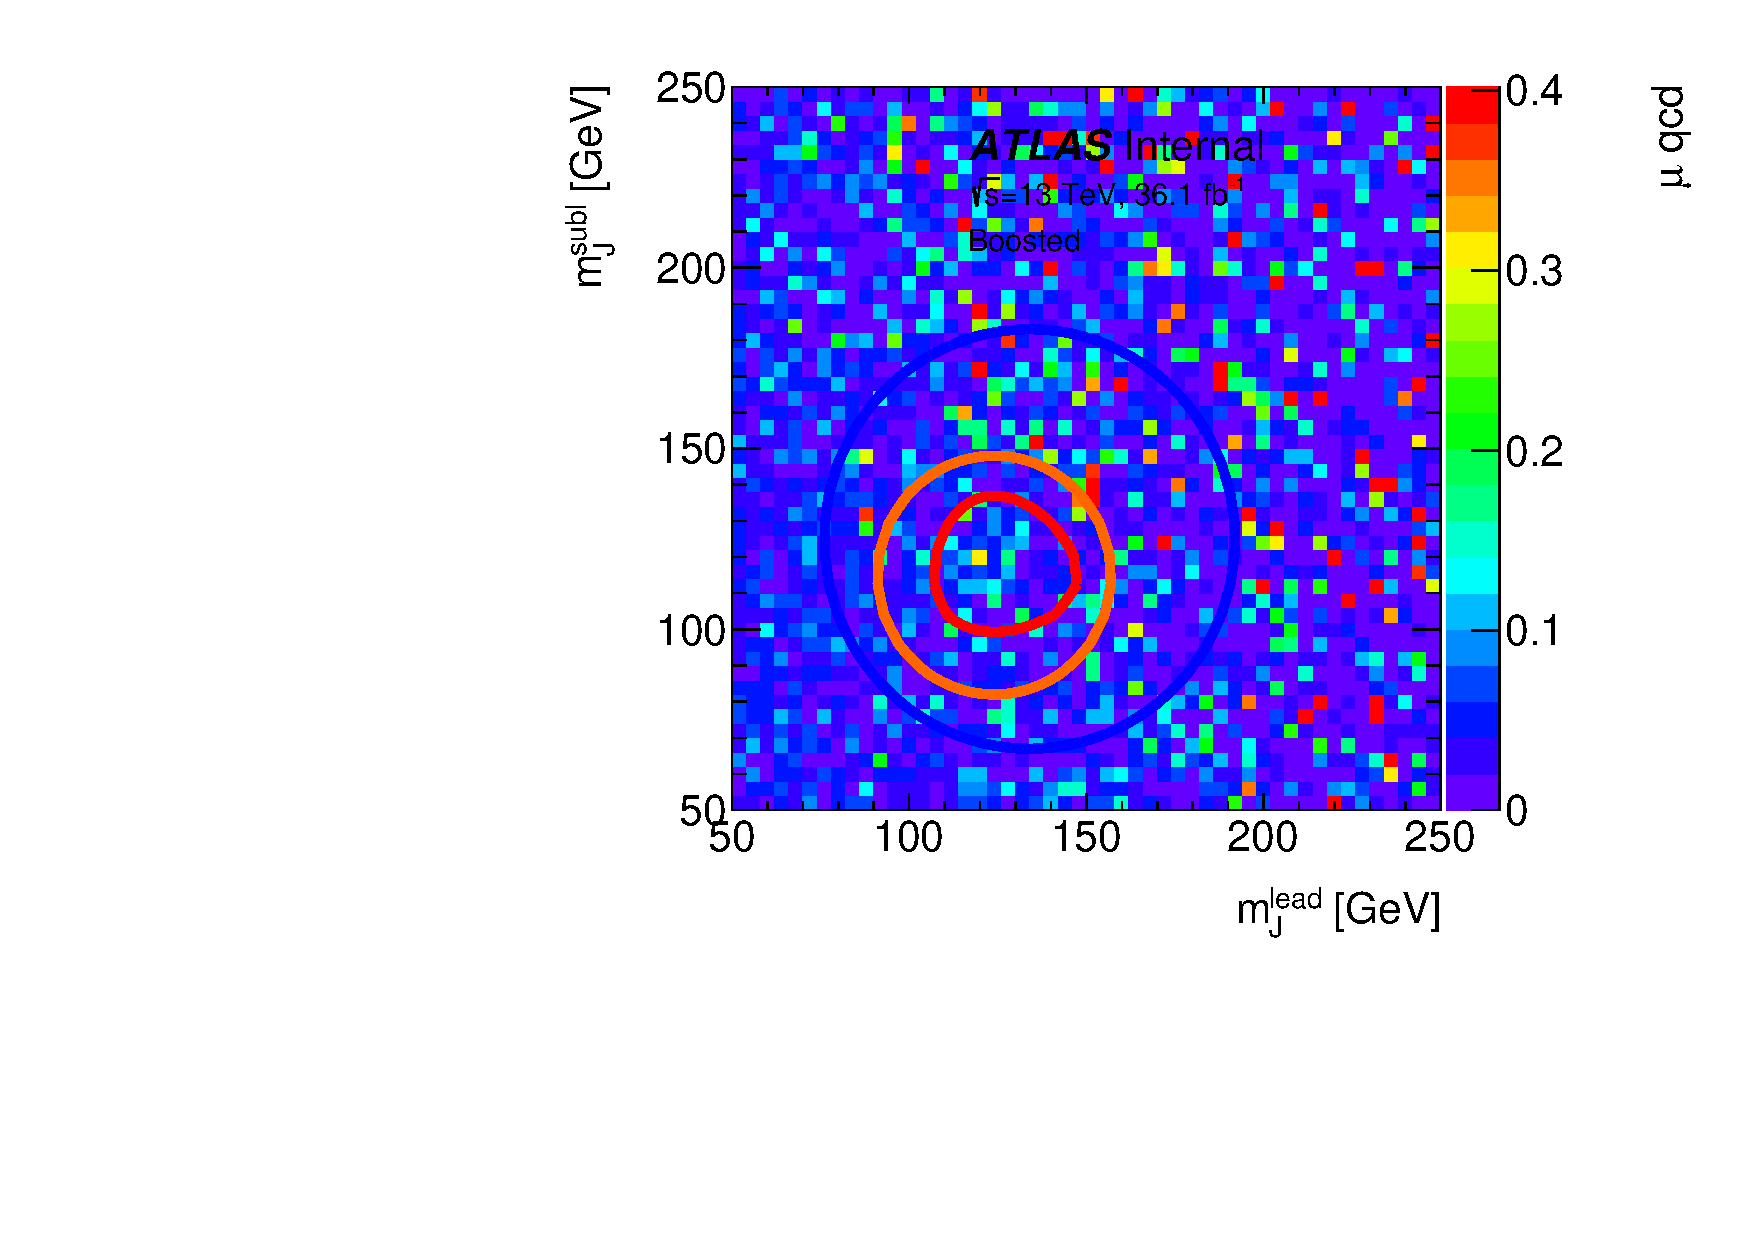
\includegraphics[width=0.31\textwidth,angle=-90]{figures/boosted/AppendixMuqcdstudy/QCD_TwoTag_split_Incl_mH0H1.pdf}
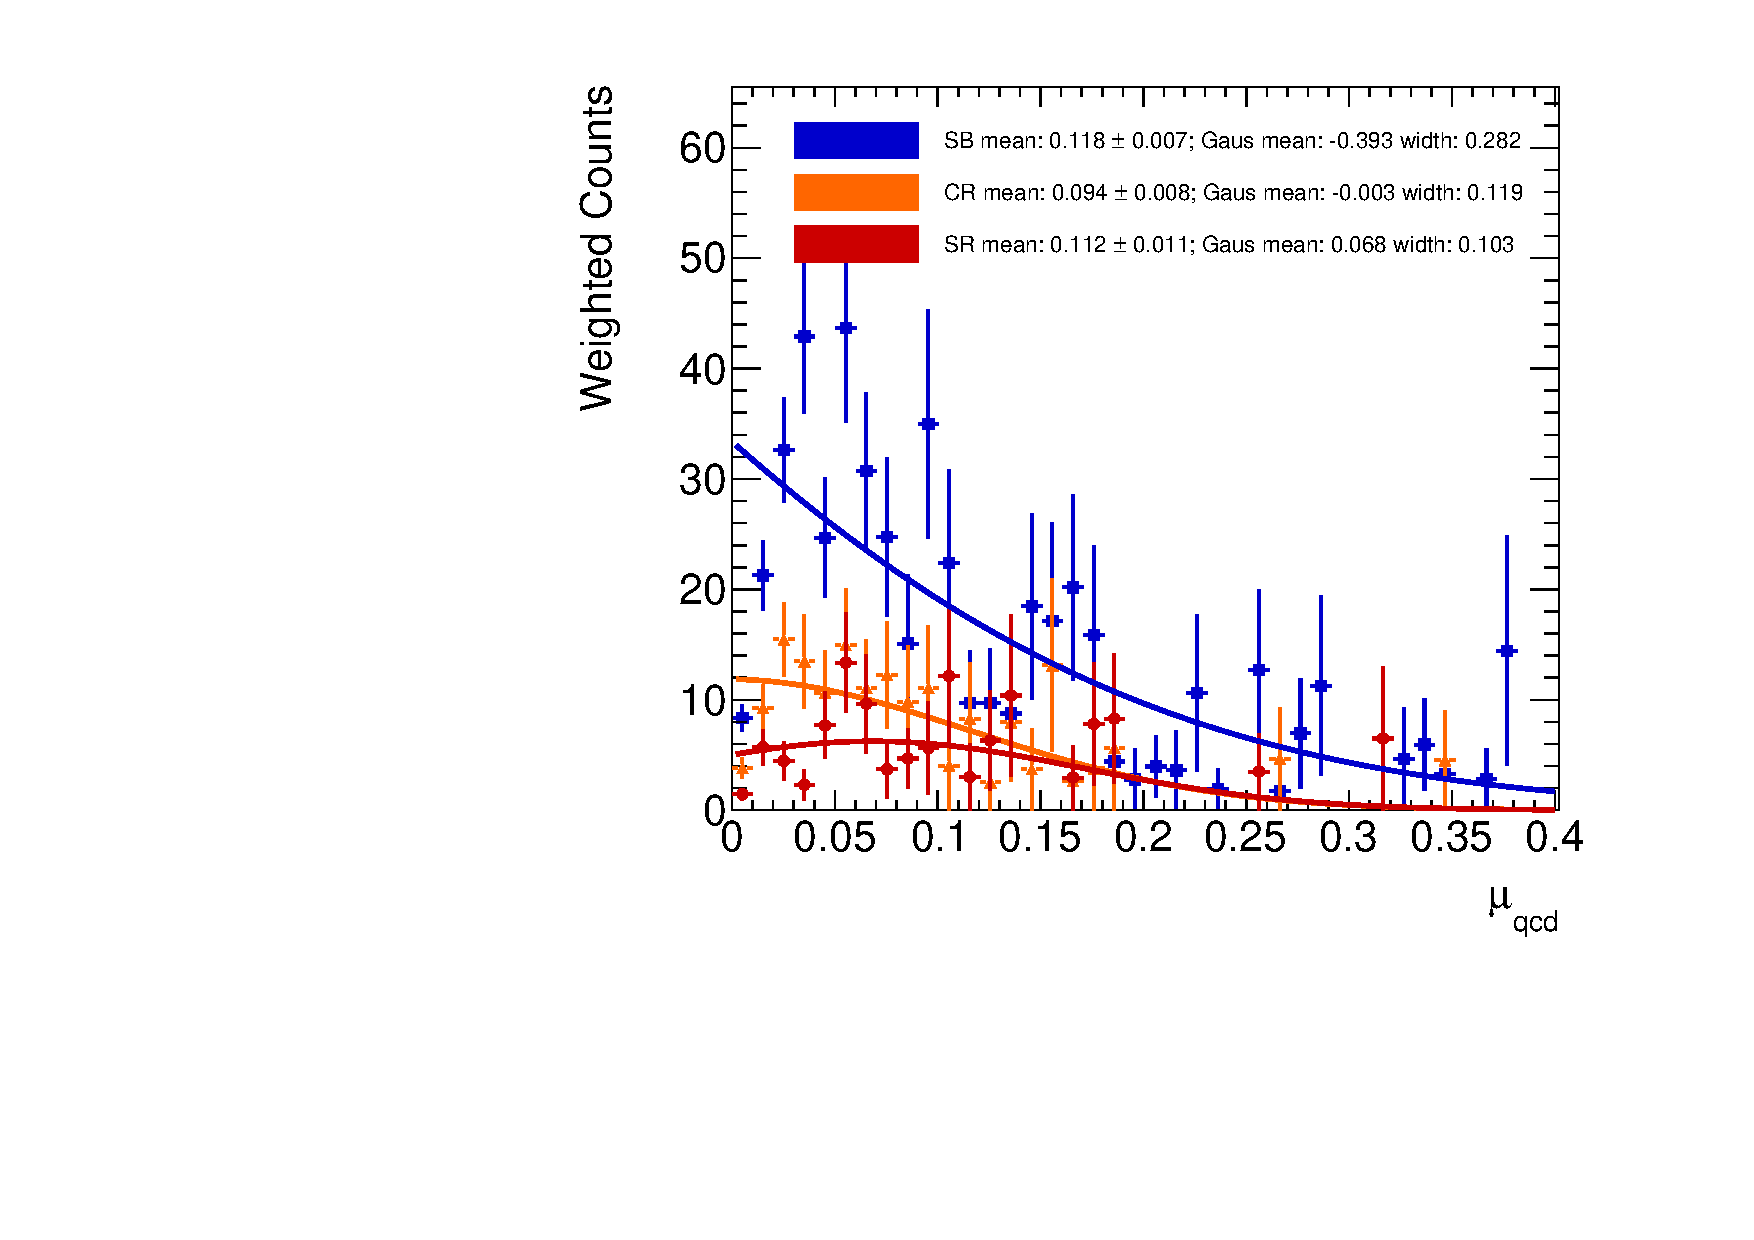
\includegraphics[width=0.31\textwidth,angle=-90]{figures/boosted/AppendixMuqcdstudy/QCD_TwoTag_split_Incl_mH0H1_pull.pdf}
\caption{$2bs$ over $1b$ \muqcd~ values in dijet MC: \muqcd variations on 2D \mleadJ-msublJ plane(left); and \muqcd pull distribution in SB/CR/SR(right), with the $N_{event}$ weighted mean value and the Guassian fit mean value shown on the plot. Poor Statistics of the dijet MC affect the pull distributions.}
\label{fig:app-muqcd-2bs-qcd}
\end{center}
\end{figure*}

\begin{figure*}[htbp!]
\begin{center}
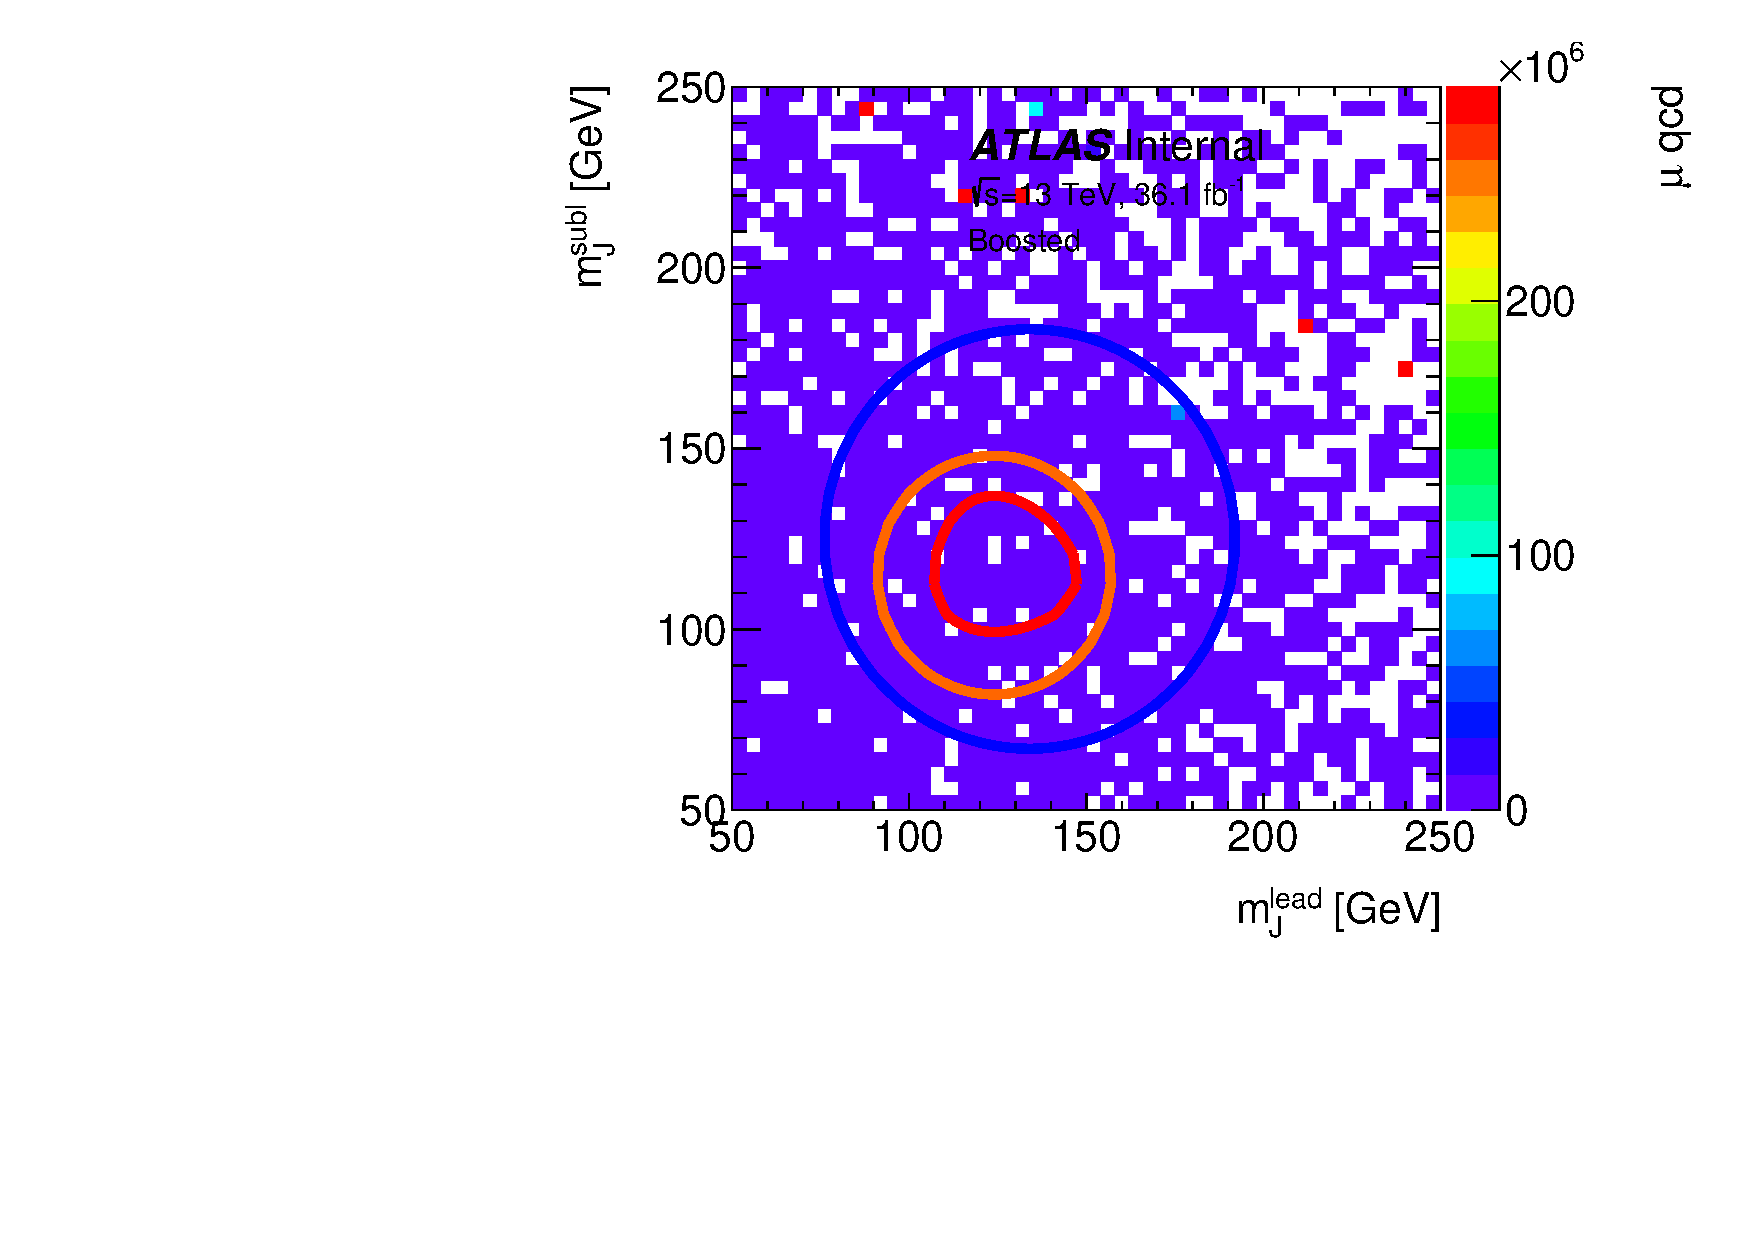
\includegraphics[width=0.31\textwidth,angle=-90]{figures/boosted/AppendixMuqcdstudy/QCD_ThreeTag_Incl_mH0H1.pdf}
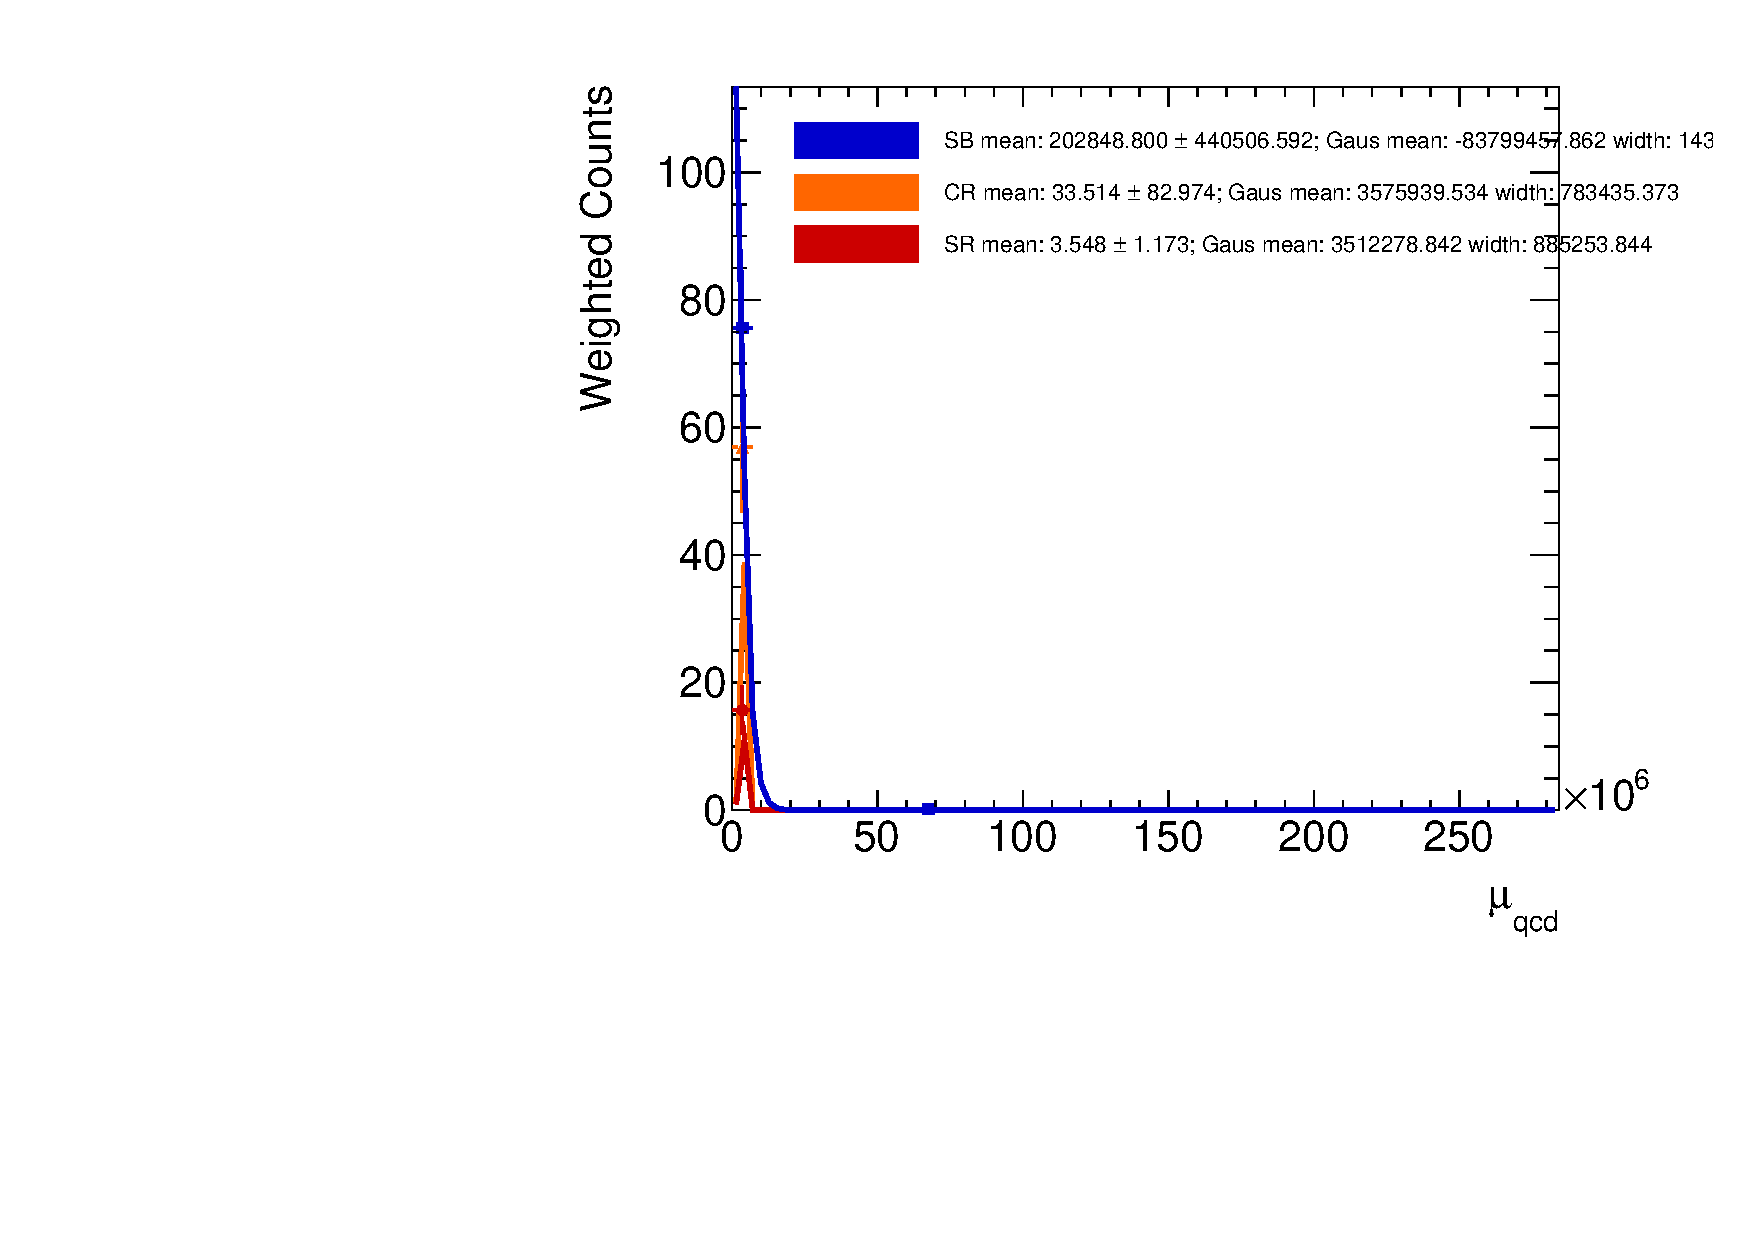
\includegraphics[width=0.31\textwidth,angle=-90]{figures/boosted/AppendixMuqcdstudy/QCD_ThreeTag_Incl_mH0H1_pull.pdf}
\caption{$3b$ over $2b$ data driven \muqcd values in dijet MC: \muqcd as a funciton of leading Higgs candidate/subleading Higgs candiate mass(left); and \muqcd value pull in Sideband/Control/Signal regions(right), with the weighted mean value and the Guassian fit mean value shown on the plot. Poor Statistics of the dijet MC affect the pull distributions.}
\label{fig:app-muqcd-3b-qcd}
\end{center}
\end{figure*}

\begin{figure*}[htbp!]
\begin{center}
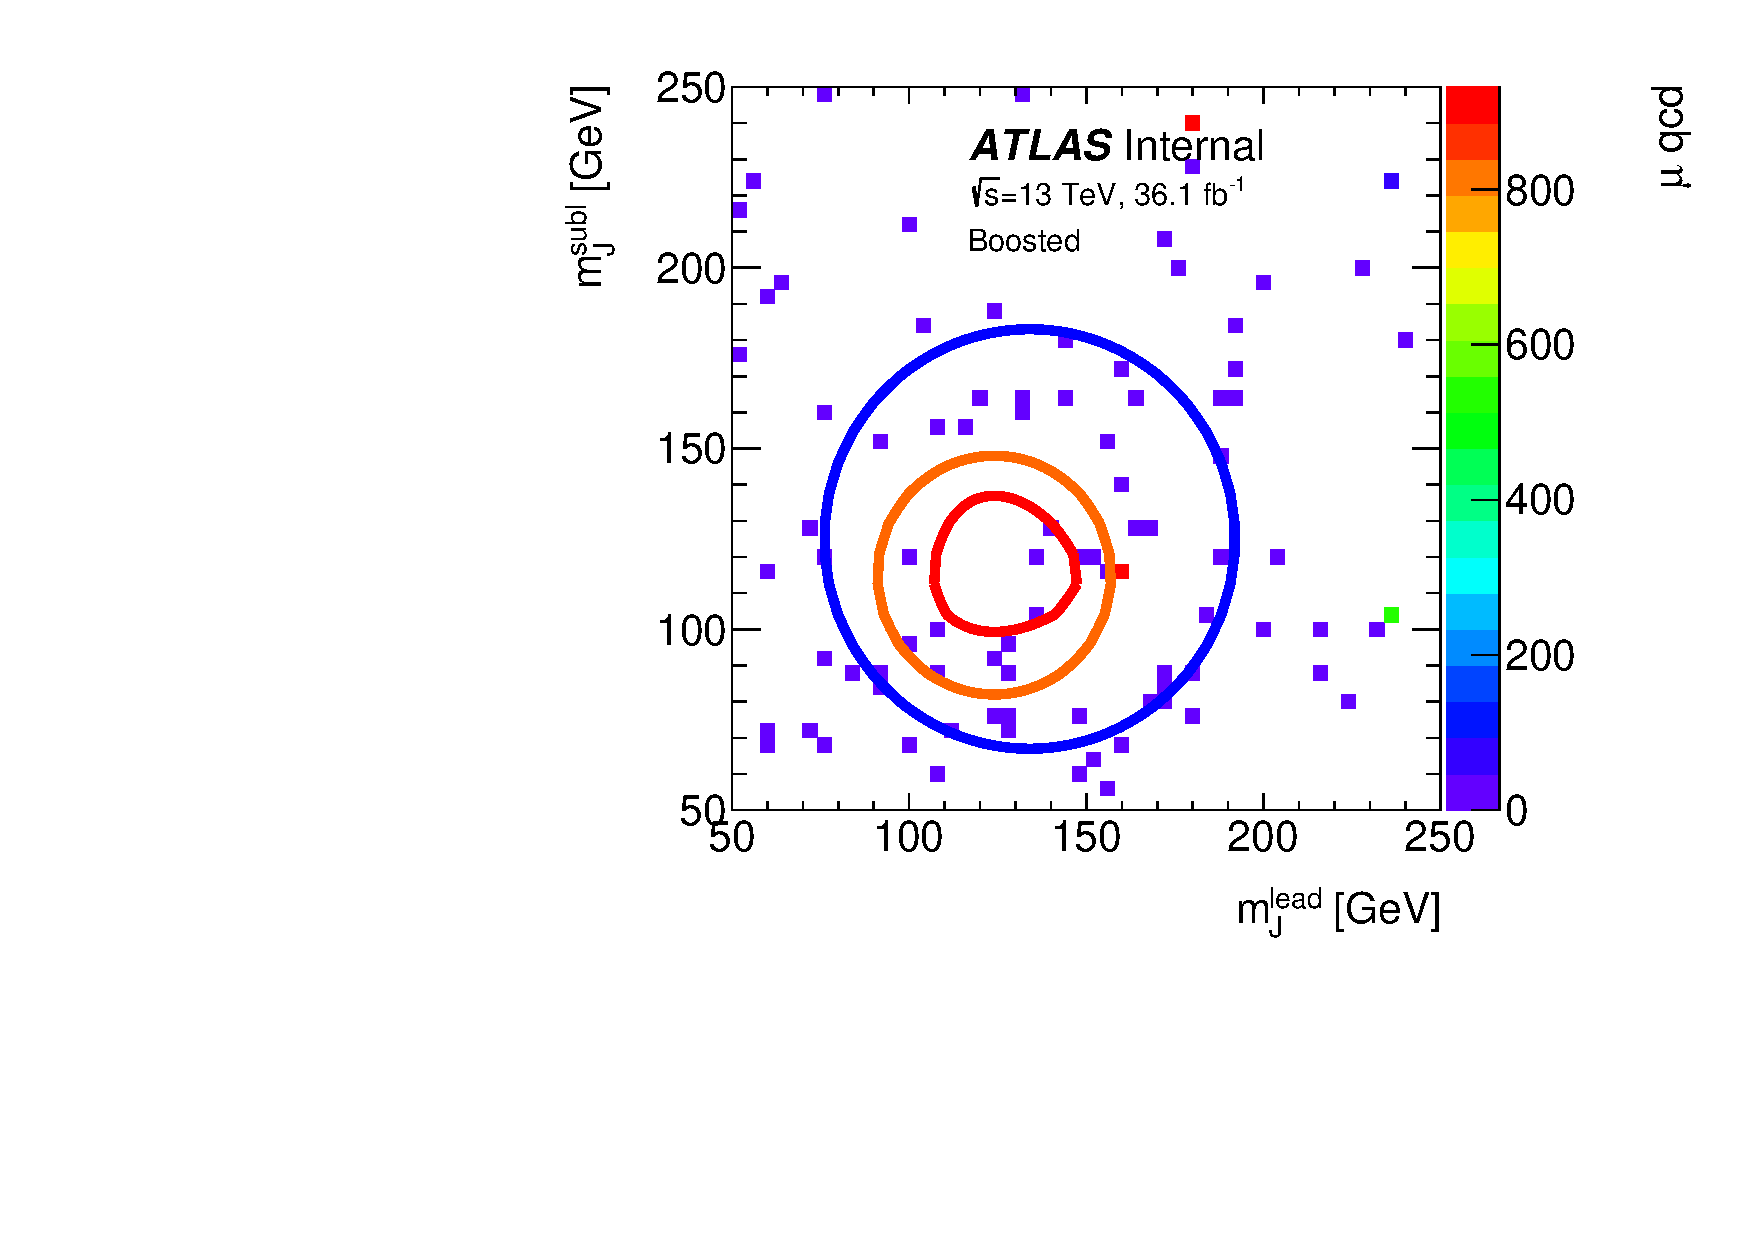
\includegraphics[width=0.31\textwidth,angle=-90]{figures/boosted/AppendixMuqcdstudy/QCD_FourTag_Incl_mH0H1.pdf}
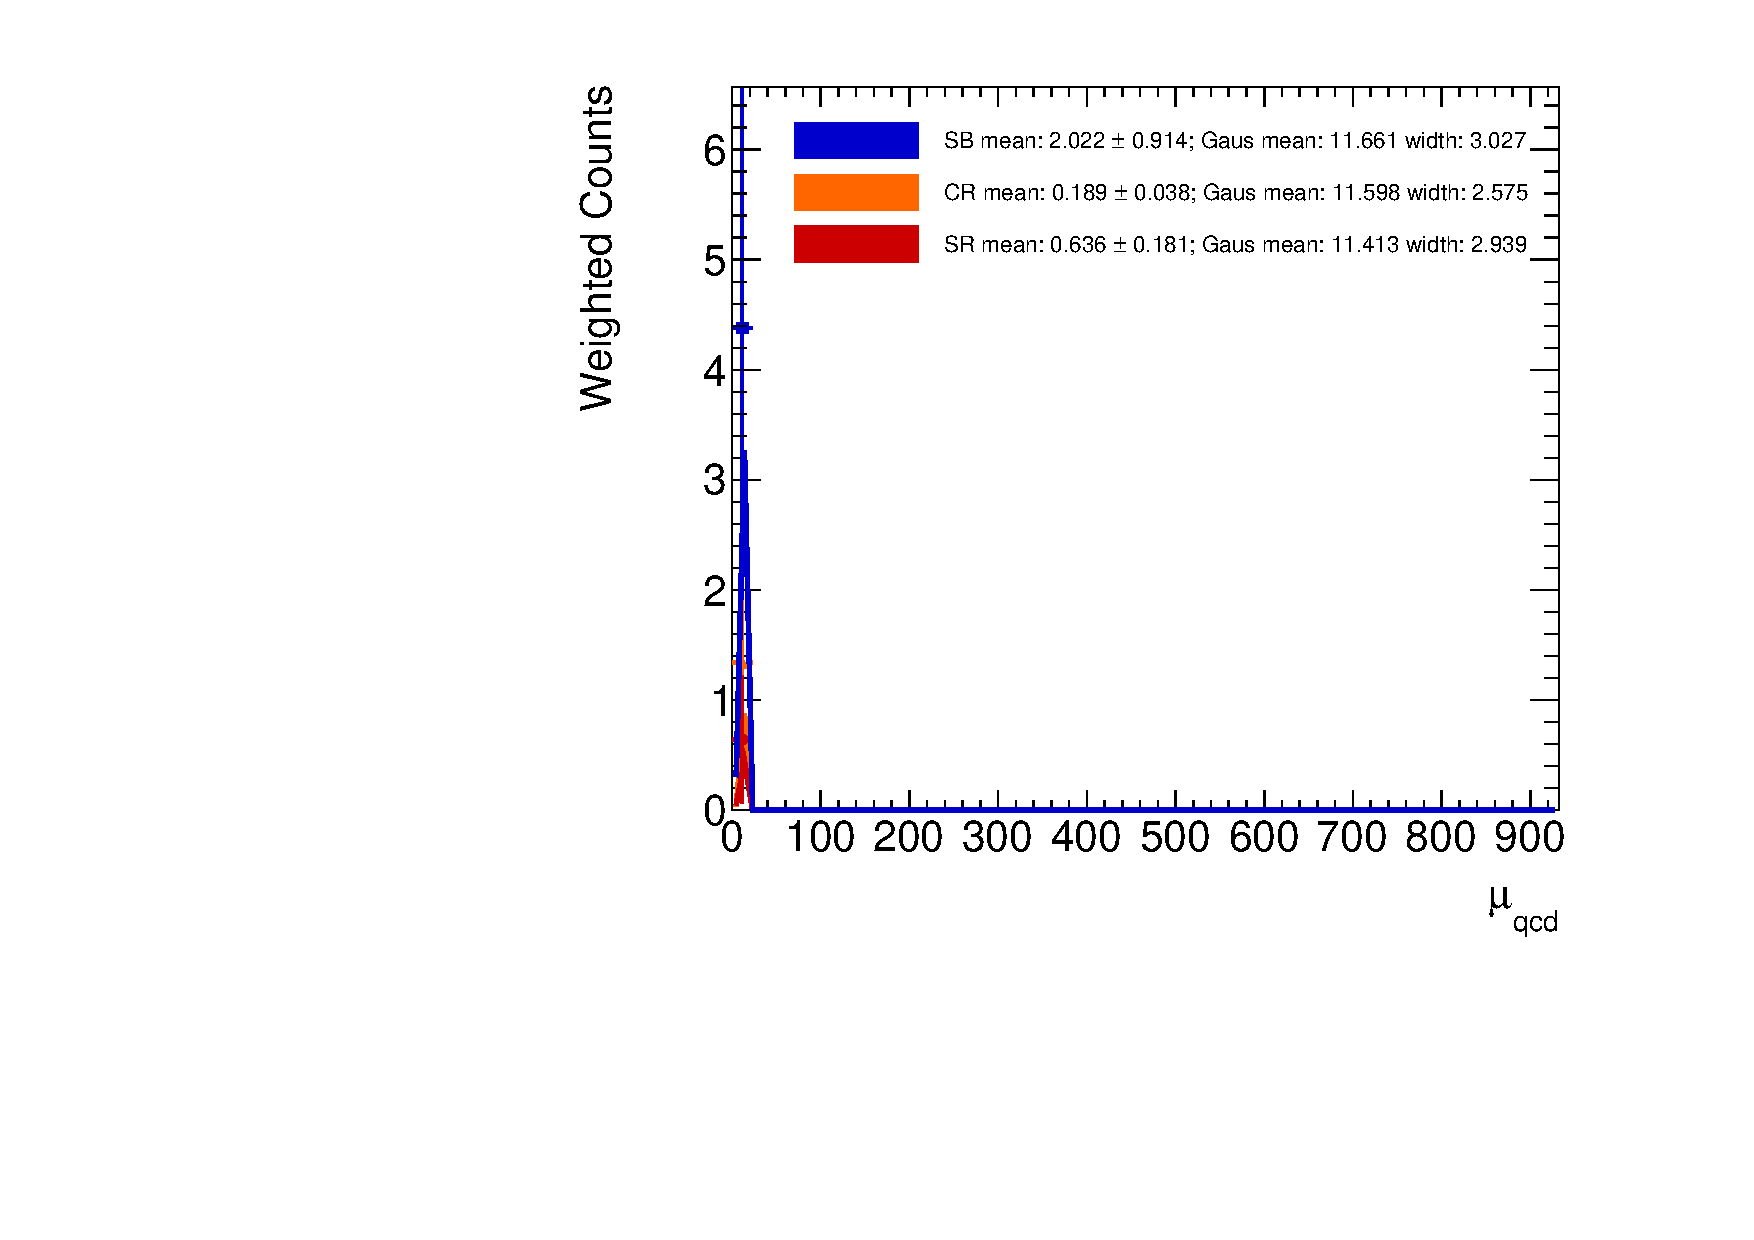
\includegraphics[width=0.31\textwidth,angle=-90]{figures/boosted/AppendixMuqcdstudy/QCD_FourTag_Incl_mH0H1_pull.pdf}
\caption{$4b$ over $2b$ data driven \muqcd values in dijet MC: \muqcd as a funciton of leading Higgs candidate/subleading Higgs candiate mass(left); and \muqcd value pull in Sideband/Control/Signal regions(right), with the weighted mean value and the Guassian fit mean value shown on the plot. Poor Statistics of the dijet MC affect the pull distributions.}
\label{fig:app-muqcd-4b-qcd}
\end{center}
\end{figure*}